\documentclass[10.5pt,scale=1.0,t,aspectratio=169,hyperref={pdfpagelabels=false}]{beamer}


\usepackage{lipsum}
\usepackage{color}
\usepackage{amsfonts}
\usepackage{amsmath,mathtools}
\usepackage{mathrsfs}
\usepackage{array}
\usepackage{algorithm}
\usepackage{hyperref}
\usepackage[spanish,es-nodecimaldot]{babel}
\usepackage[utf8]{inputenc}
\usepackage{graphicx}
\usepackage{multicol}
\usepackage{multirow}
\usepackage{enumitem}
\usepackage[document]{ragged2e}
\usepackage[absolute,overlay]{textpos}
\textblockorigin{0mm}{0mm} 
\usefonttheme[onlymath]{serif}
\usepackage{verbatim}
\usepackage{cite}
\usepackage{multicol}
\usepackage{siunitx}




\newenvironment{conditions}[1][where:]
{#1 \begin{tabular}[t]{>{$}l<{$} @{${}={}$} l}}
	{\end{tabular}\\[\belowdisplayskip]}


\newcolumntype{L}{>{$}l<{$}} % math-mode version of "l" column type


\newcounter{saveenumi}
\newcommand{\seti}{\setcounter{saveenumi}{\value{enumi}}}
\newcommand{\conti}{\setcounter{enumi}{\value{saveenumi}}}

\setbeamertemplate{bibliography item}{\insertbiblabel}


\hypersetup{colorlinks=true,
	linkcolor=blue,
	linktoc=all,				
	citecolor=blue,
	urlcolor=red,
	pdftitle={ELECTRONICA DIGITAL},
	pdfauthor={Santiago Rúa Pérez},
	pdfcreator={Santiago Rúa Pérez}}


\definecolor{GreenDark}{rgb}{0.0, 0.60, 0.0}
\definecolor{RedDark}{rgb}{183, 0.0, 0.0}
\definecolor{BlueDark}{rgb}{0.0, 0.0, 167}
\definecolor{BlueLight}{rgb}{0.2, 0.451, 0.517}


\graphicspath{{imag/}}

\newcommand{\Ho}{$H_{0}$}
\newcommand{\Ha}{$H_{a}$}
\newcommand{\Nota}{{\bf Nota: }}
\newcolumntype{P}[1]{>{\centering\arraybackslash}p{#1}}
\newcolumntype{M}[1]{>{\centering\arraybackslash}m{#1}}

\newcommand{\less}{<}
\newcommand{\greater}{>}


\setlength{\parindent}{1em}
\setlength{\parskip}{.6em}
\renewcommand{\baselinestretch}{.9}

%%%%    C environment    ---------------- %%%%%%%%%%%%%%%.
\usepackage{listings}
\usepackage{xcolor}
\definecolor{mGreen}{rgb}{0,0.6,0}
\definecolor{mGray}{rgb}{0.5,0.5,0.5}
\definecolor{mPurple}{rgb}{0.58,0,0.82}
\definecolor{backgroundColour}{rgb}{0.95,0.95,0.92}

\lstdefinestyle{CStyle}{
	backgroundcolor=\color{backgroundColour},   
	commentstyle=\color{mGreen},
	keywordstyle=\color{magenta},
	numberstyle=\tiny\color{mGray},
	stringstyle=\color{mPurple},
	basicstyle=\tiny,
	breakatwhitespace=false,         
	breaklines=true,                 
	captionpos=b,                    
	keepspaces=true,                 
	numbers=left,                    
	numbersep=5pt,                  
	showspaces=false,                
	showstringspaces=false,
	showtabs=false,                  
	tabsize=2,
	language=C
}
%%--------------------------------------------------------------------------


\title{Electrónica Digital II}   
\author{Santiago Rúa Pérez, PhD.} 
\date{\today} 

\setlength{\TPHorizModule}{\textwidth}
\setlength{\TPVertModule}{\textwidth}

\newcommand{\btVFill}{\vskip0pt plus 1filll}


\setbeamertemplate{sidebar right}{}
\setbeamertemplate{footline}
{
	\leavevmode%
	\hbox{%
		\begin{beamercolorbox}[wd=.333333\paperwidth,ht=2.25ex,dp=1ex,center]{author in head/foot}%
			\usebeamerfont{author in head/foot}\insertshortauthor
		\end{beamercolorbox}%
		\begin{beamercolorbox}[wd=.333333\paperwidth,ht=2.25ex,dp=1ex,center]{title in head/foot}%
			\usebeamerfont{title in head/foot}\insertshorttitle
	\end{beamercolorbox}}%
	\vskip0pt%
}
\makeatother

\begin{document}
	%%%%%%%%%%%%%%%%%% FRAME %%%%%%%%%%%%%%%%%%%%%%%%%%
	\begin{frame}
		\titlepage
	\end{frame}
	%%%%%%%%%%%%%%%%% FRAME START %%%%%%%%%%%%%%%%%%%%%%%%%%
	\frame{
		%\frametitle{}
		\begin{center}
			\LARGE \textcolor{blue}{COMUNICACIONES SERIALES}
		\end{center}
		
	}
	
	%%%%%%%%%%%%%%%%% FRAME %%%%%%%%%%%%%%%%%%%%%%%%%%

%%%%%%%%%%%%%%%%% FRAME %%%%%%%%%%%%%%%%%%%%%%%%%%
\begin{frame}
\frametitle{Panorama general}
\begin{itemize}
\item Comunicaciones seriales
\begin{itemize}
	\item Conceptos
	\item Herramientas
	\item Software: polling, interrupciones y buffering
\end{itemize}
\item Comunicaciones SPI
\begin{itemize}
	\item Conceptos
	\item Periféricos del K64
\end{itemize}
\item Comunicaciones I$^2$C
\begin{itemize}
	\item Conceptos
	\item Periféricos del K64
\end{itemize}
\item Comunicaciones UART
\begin{itemize}
	\item Conceptos
	\item Periféricos del K64
\end{itemize}
\end{itemize}
\end{frame}
%%%%%%%%%%%%%%%%% FRAME %%%%%%%%%%%%%%%%%%%%%%%%%%
\begin{frame}
	\frametitle{Porque comunicaciones seriales?}
	\begin{columns}
		\column{0.7\linewidth}
		
		\begin{itemize}
			\item Aunque el tamaño de la palabra nativa para la CPU es de 32 bits, enviar todos los bits de una palabra simultáneamente tiene desventajas:
			\begin{itemize}
				\item \textbf{Costo y peso}: paquete CI más grande, más cables, conectores más grandes
				\item \textbf{Fiabilidad mecánica}: más cables implican más contactos de conexión para fallar
				\item \textbf{Complejidad de sincronización}: algunos bits pueden llegar más tarde que otros debido a variaciones en la capacitancia y la resistencia a través de los conductores.
				\item \textbf{Complejidad y potencia del circuito}: es posible que no desee tener 16 transmisores + receptores diferentes en el sistema
			\end{itemize}
			\item La comunicación serial reduce el numero de señales requeridas
		\end{itemize}
		
		
		\column{0.3\linewidth}
		
		\begin{figure}
			\centering
			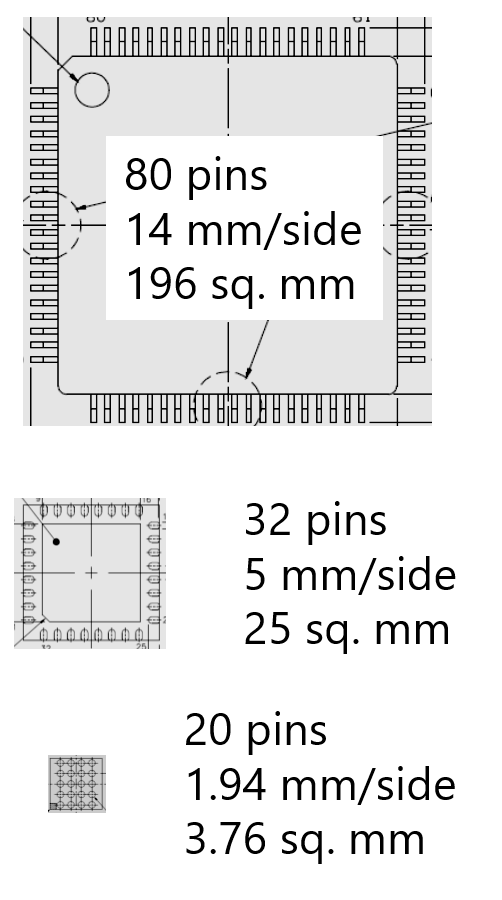
\includegraphics[scale=0.35]{01_Packages}
		\end{figure}
	\end{columns}
\end{frame}
%%%%%%%%%%%%%%%%% FRAME %%%%%%%%%%%%%%%%%%%%%%%%%%
\begin{frame}
	\frametitle{Ejemplo de sistema}
		
	\begin{figure}
		\centering
		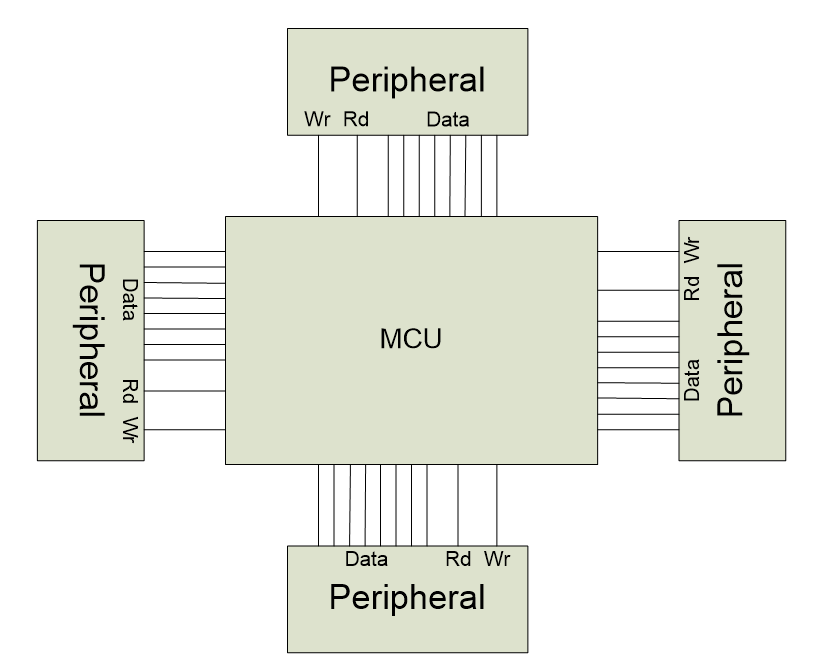
\includegraphics[scale=0.35]{02_Example1}
	\end{figure}
	
	\begin{itemize}
		\item Conexiones dedicas punto a punto
		\begin{itemize}
			\item Linea de datos paralelas, lineas de lectura y escritura entre el MCU y cada periféricos.
		\end{itemize}
		\item Rápido, permite transferencias simultáneas
		\item Requiere muchas conexiones, area de PCB, y escalamiento malo.
		\begin{itemize}
			\item Se necesitarian $4*(8+2)=40$ pines para el MCU solo comunicarse. 	
		\end{itemize}
	\end{itemize}

\end{frame}

%%%%%%%%%%%%%%%%% FRAME %%%%%%%%%%%%%%%%%%%%%%%%%%
\begin{frame}
	\frametitle{Buses paralelos}
	
	\begin{figure}
		\centering
		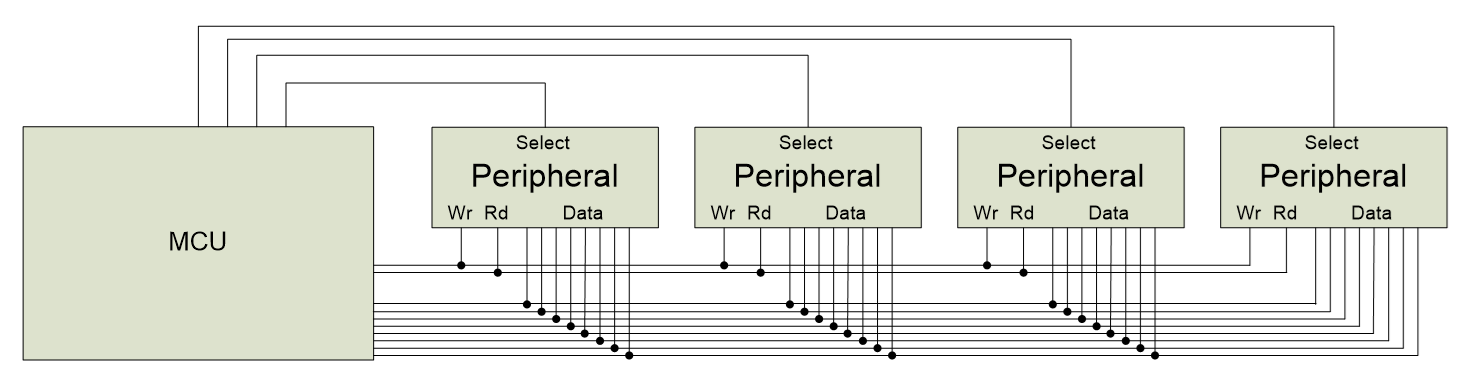
\includegraphics[scale=0.4]{03_BusParalell}
	\end{figure}
	
	\begin{itemize}
		\item Todos los dispositivos utilizan un bus para compartir datos, escribir y leer señales.
		\item El MCU utiliza lineas individuales para seleccionar el periférico con el que se está comunicando.
		\item El MCU requiere menos pines de datos, pero de todas formas uno por bit.
		\begin{itemize}
			\item Se requieren $4+(8+2)=14$ pines para comunicarse.
		\end{itemize}
		\item El MCU puede comunicarse con un periférico al tiempo. 
	\end{itemize}
	
\end{frame}

%%%%%%%%%%%%%%%%% FRAME %%%%%%%%%%%%%%%%%%%%%%%%%%
\begin{frame}
	\frametitle{Transmisión de datos serial sincrónica}
	
	\begin{figure}
		\centering
		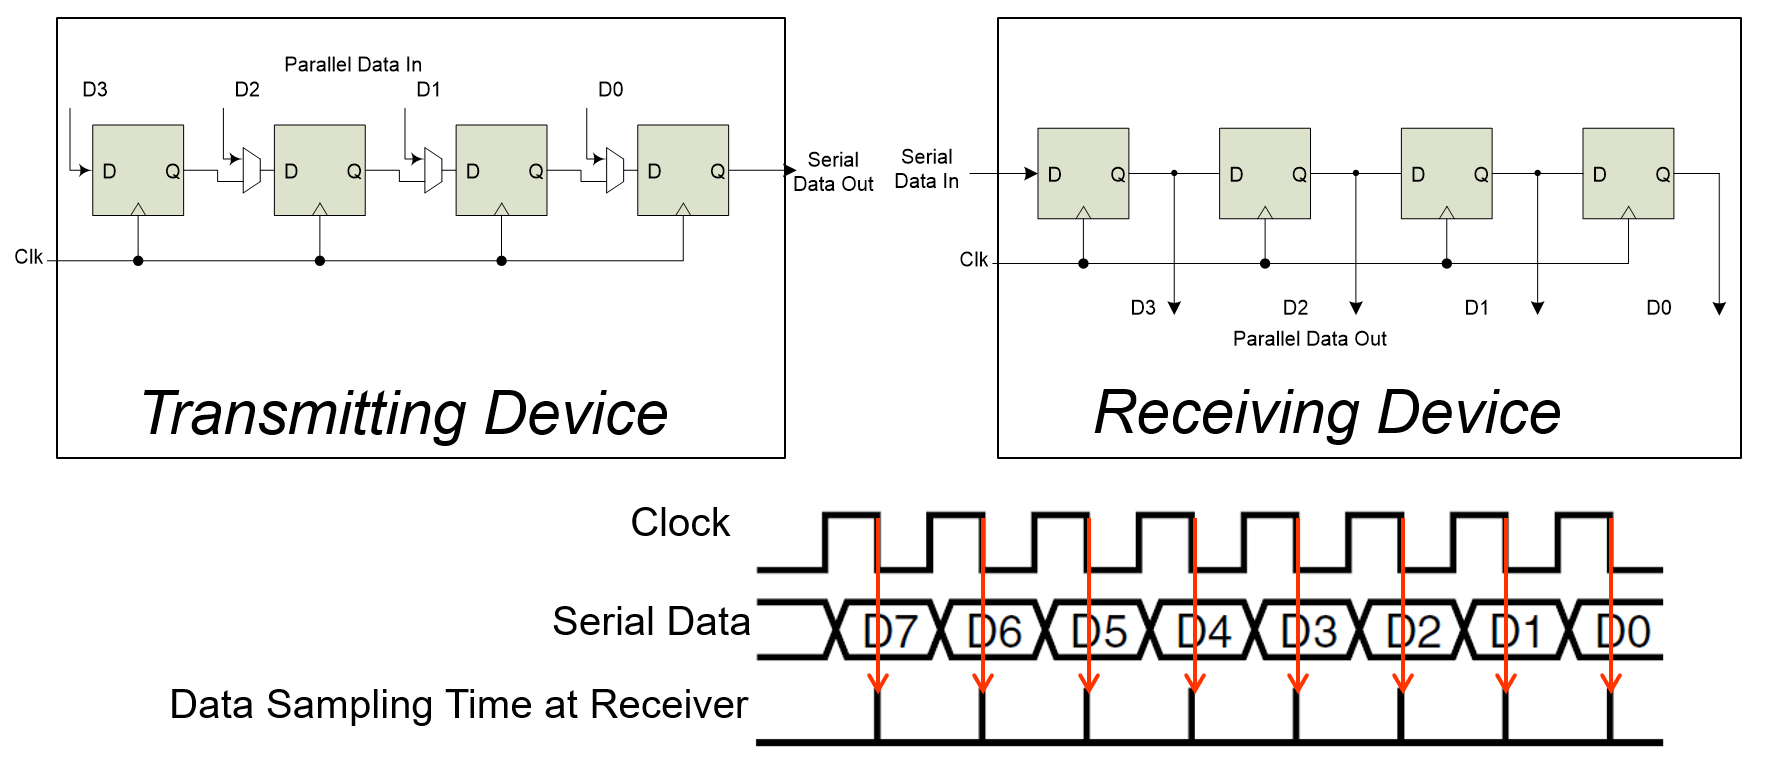
\includegraphics[scale=0.4]{04_SyncSerial}
	\end{figure}
	
	\begin{itemize}
		\item Utiliza registros de desplazamiento y señales de clock para convertir formatos seriales y paralelos
		\item Sincrónica: una señal de reloj está de forma explicita acompañando a los datos. 
	\end{itemize}
	
\end{frame}

%%%%%%%%%%%%%%%%% FRAME %%%%%%%%%%%%%%%%%%%%%%%%%%
\begin{frame}
	\frametitle{Transmisión de datos serial sincrónica full duplex}
	
	\begin{figure}
		\centering
		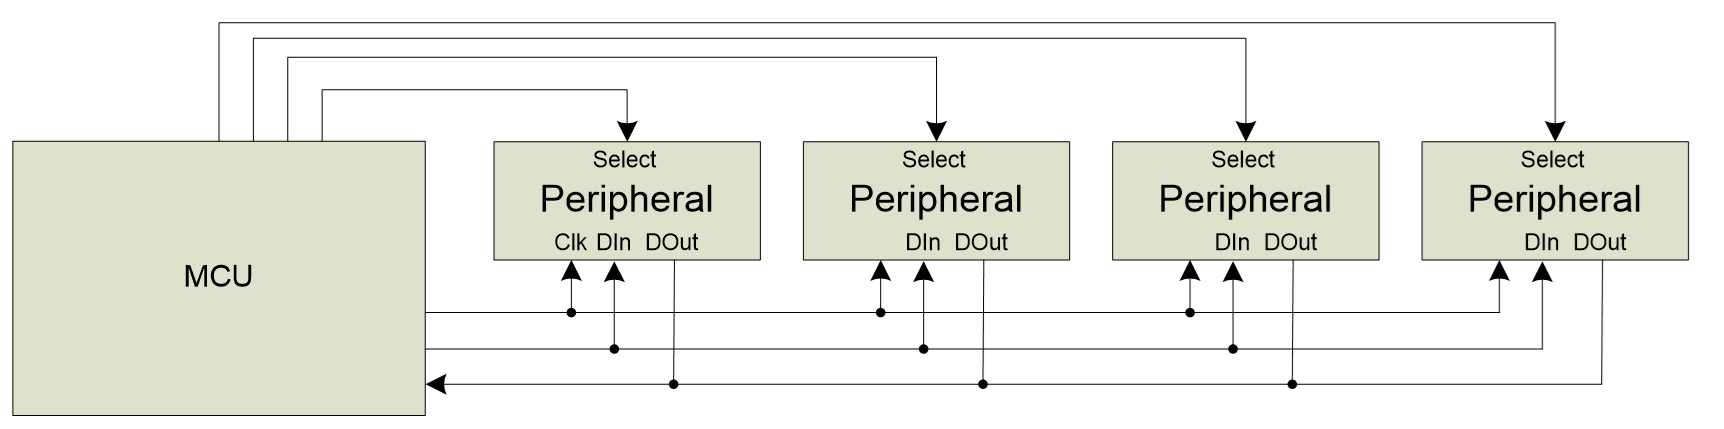
\includegraphics[scale=0.4]{05_SyncSerialFullDuplex}
	\end{figure}
	
	\begin{itemize}
		\item Ahora se utilizan dos lineas seriales - una para lectura y otra para escritura
		\begin{itemize}
			\item Permite simultáneamente tener envió y recepción de datos 
			\item Se requiere $4+3=7$ pines del MCU para comunicarse. 
		\end{itemize}
	\end{itemize}
	
\end{frame}

%%%%%%%%%%%%%%%%% FRAME %%%%%%%%%%%%%%%%%%%%%%%%%%
\begin{frame}
	\frametitle{Transmisión de datos serial sincrónica half duplex}
	
	\begin{figure}
		\centering
		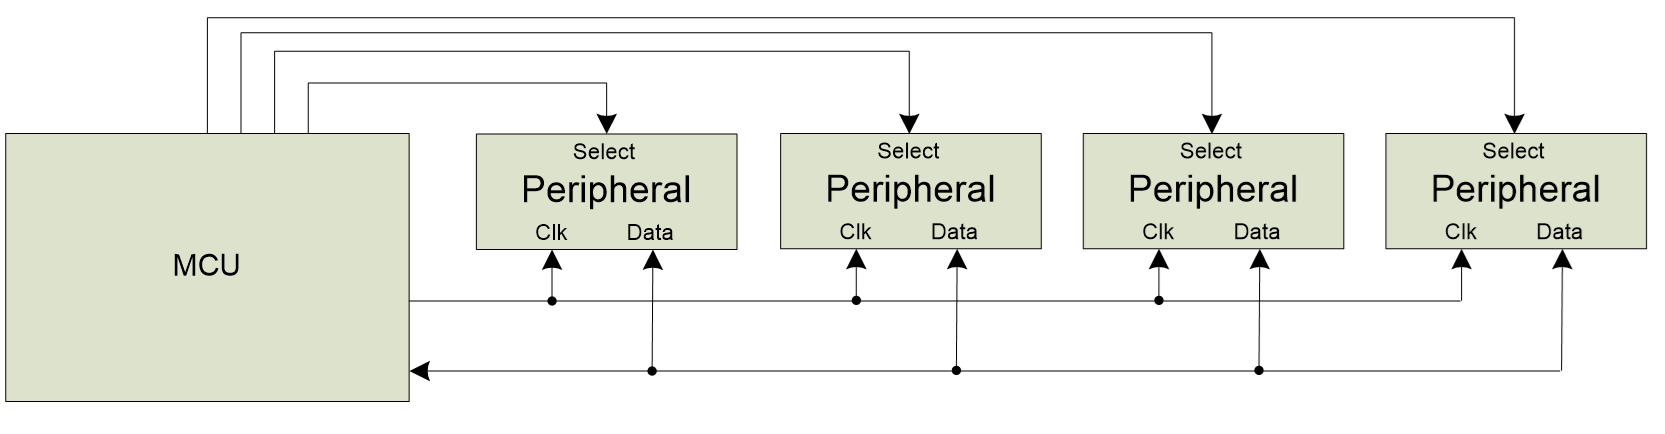
\includegraphics[scale=0.4]{06_SyncSerialHalfDuplex}
	\end{figure}
	
	\begin{itemize}
		\item Se comparten la linea de datos serial
		\begin{itemize}
			\item Se requiere $4+2=6$ pines del MCU para comunicarse. 
		\end{itemize}
		\item No se permite envió y recepción de datos simultáneamente. 
	\end{itemize}
	
\end{frame}

%%%%%%%%%%%%%%%%% FRAME %%%%%%%%%%%%%%%%%%%%%%%%%%
\begin{frame}
	\frametitle{Transmisión de datos serial asincrónica}
	
	\begin{figure}
		\centering
		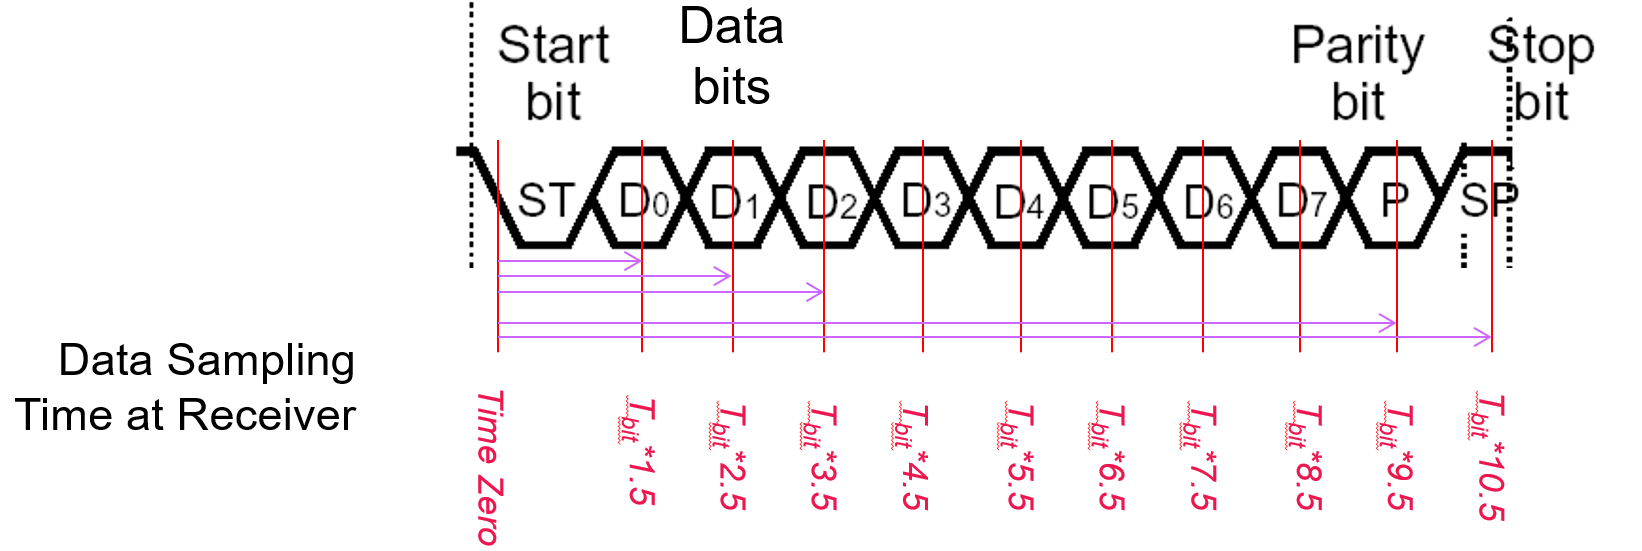
\includegraphics[scale=0.4]{07_AsyncSerial}
	\end{figure}
	
	\begin{itemize}
		\item Se elimina la linea de clock
		\item El transmisor y el receptor deben generar su clock local
		\item El transmisor debe adicionar un bit de start para indicar el inicio de una comunicación.
		\item El receptor detectar ese cambio de flanco, luego utiliza su referencia de tiempo para muestrear cada linea y extraer cada bit $N$ en el tiempo $T_{bit}*(N+1.5)$
		\item El bit de stop es usado para detectar errores de tiempo. 
	\end{itemize}
	
\end{frame}

%%%%%%%%%%%%%%%%% FRAME %%%%%%%%%%%%%%%%%%%%%%%%%%
\begin{frame}
	\frametitle{Especificaciones de la comunicaciones seriales}
	\begin{itemize}
		\item Campos del data frame
		\begin{itemize}
			\item Bit de start (un bit)
			\item Datos (LSB a MSB): tamaños de 7, 8 y 9 bits.
			\item Bit opcional de paridad para detección de errores.
			\item Bit de stop, uno o dos bits.
		\end{itemize}
		\item Todos los dispositivos deben usar la misma configuración
		\begin{itemize}
			\item Eg: velocidades de comunicación de 300, 600, 1200, 2400, 9600, 14400, 19200 baud
		\end{itemize}
		\item Protocolos sofisticados tienen mayor información el los data frame
		\begin{itemize}
			\item Control de acceso al medio: cuando múltiples nodos están en el mismo bus, deben arbitrar para solicitar permisos de transmisión.
			\item Información de direccionamiento: para cual nodo se pretenden mandar la información?
			\item Carga útil más grande
			\item Detección de errores superior, o información para corrección.
			\item Solicitud para respuesta inmediata
		\end{itemize}
	\end{itemize}
	
\end{frame}

%%%%%%%%%%%%%%%%% FRAME %%%%%%%%%%%%%%%%%%%%%%%%%%
\begin{frame}
	\frametitle{Detección de errores}
	\begin{itemize}
		\item Puede ser enviada información adicional para verificar que los datos fueron recibidos apropiadamente
		\item Se necesita especificar que tipo de paridad se espera: par, impar o ninguna
		\item El bit de paridad se pone 1 de tal forma que la cantidad total sea par (para paridad par) o impar (para paridad impar)
		\begin{itemize}
			\item $01110111$ tiene en total 6 bits en 1, entonces el bit de paridad se pone en 1 si se quiere paridad impar y 0 si se quiere par.
			\item $01100111$ tiene en total 5 bits en 1, entonces el bit de paridad se pone en 0 si se quiere paridad impar y 1 si se quiere par.
		\end{itemize}
		\item El bit de paridad puede detectar errores si 1, 3, 5, 7 o 9 bits están corruptos, pero no detecta bits corruptos pares.
		\item Códigos de detección de errores mas fuertes existen (Cyclic redundancy Check CRC) y utilizan múltiples bits, lo que pueden ayudar a detectar más errores. 
		\begin{itemize}
			\item Usado en buses CAN, USB, Ethernet, Bluetooth, etc
		\end{itemize}
	\end{itemize}
	
\end{frame}

%%%%%%%%%%%%%%%%% FRAME %%%%%%%%%%%%%%%%%%%%%%%%%%
\begin{frame}
	\frametitle{Arquitectura de software para manejo de comunicaciones asincrónicas}
	
	\begin{itemize}
		\item La comunicación es asincrónica para el programa
		\begin{itemize}
			\item No se sabe que código esta ejecutando el programa cuando se reciben datos.
			\item No se sabe cuando llega el próximo dato
			\item No se sabe cuando el dato de salida se completa
			\item Cuando ocurre un error
			\item Se necesita algún tipo de sincronización entre el programa y la interfaz serial. 
		\end{itemize}
		\item Opciones
		\begin{itemize}
			\item Polling
			\begin{itemize}
				\item Esperar hasta que el dato este disponible
				\item Sencillo pero ineficiente
			\end{itemize}
			\item Interrupción
			\begin{itemize}
				\item La CPU interrumpe el programa cuando el dato está disponible
				\item Eficiente, pero no complejo
			\end{itemize}
		\end{itemize}
	\end{itemize}	
\end{frame}
%%%%%%%%%%%%%%%%% FRAME %%%%%%%%%%%%%%%%%%%%%%%%%%
\begin{frame}
	\frametitle{Comunicaciones seriales e interrupciones}
	\begin{columns}
		\column{0.6\linewidth}
		
		\begin{itemize}
			\item Se desea tener múltiples hilos de control en el programa
			\begin{itemize}
				\item Programa principal
				\item ISR
				\begin{itemize}
					\item Transmitir la actividad del ISR - se ejecuta cuando la interfaz serial está lista para mandar otro carácter.
					\item Recibir la actividad ISR - ejecuta el serial cuando recibe un carácter. 
					\item Error en el ISR - ejecuta si hay un error.
				\end{itemize}
			\end{itemize}
			\item Se necesita una forma de bufferear la información entre hilos. 
			\begin{itemize}
				\item Solución: cola circular con punteros de cabeza y cola.
				\item Uno para Tx, y otro para Rx.
			\end{itemize}
		\end{itemize}
		
		
		\column{0.4\linewidth}
		
		\begin{figure}
			\centering
			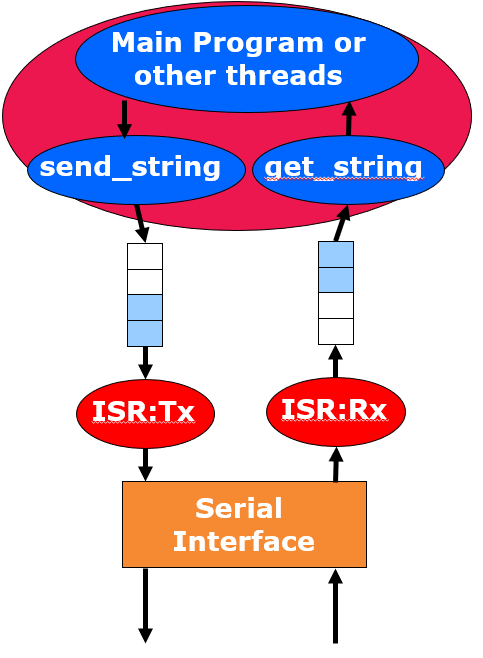
\includegraphics[scale=0.35]{08_SerialInterrupt}
		\end{figure}
	\end{columns}
\end{frame}

%%%%%%%%%%%%%%%%% FRAME %%%%%%%%%%%%%%%%%%%%%%%%%%
\begin{frame}
	\frametitle{Conexiones al ISR}
	\begin{columns}
		\column{0.6\linewidth}
		\begin{itemize}
			\item El ARM Cortex-M4 tiene dos IRQ para cada interfaz serial de comunicación. 
			\item Dentro del ISR se necesita determinar que disparo la atención al servicio de la interrupción. 
		\end{itemize}
		
		
		\column{0.4\linewidth}
		\begin{figure}
			\centering
			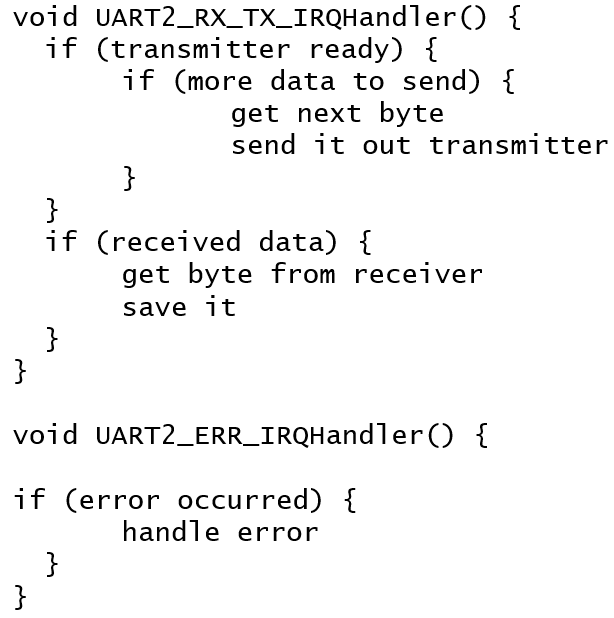
\includegraphics[scale=0.35]{09_ISRIRQ}
		\end{figure}
	\end{columns}
\end{frame}
%%%%%%%%%%%%%%%%% FRAME %%%%%%%%%%%%%%%%%%%%%%%%%%
\begin{frame}
	\frametitle{Código para implementar colas}
	{\small
	\begin{columns}
		\column{0.6\linewidth}
		\begin{itemize}
			\setlength\itemsep{0em}
			\item \textbf{Enqueue}: el puntero \texttt{tail\_ptr} apunta a la siguiente entrada libre (cola). Aquí debe ingresar el nuevo item.
			\item \textbf{Dequeue}: el puntero \texttt{head\_ptr} apunta al item a retirar (cabeza).
			\item \texttt{\#define} para el tamaño de la cola 
			\item Una cola por dirección
			\begin{itemize}
				\setlength\itemsep{0em}
				\item ISR saca datos \texttt{tx\_q} para transmitir
				\item ISR carga datos \texttt{rx\_q} para recibir.
			\end{itemize}
			\item Otro hilos cargar y descargan datos de las colas.
			\item Se necesita ajustar el puntero al final del buffer para volverlo circular
			\begin{itemize}
				\item Usar el operado módulo (\%) si el tamaño de la cola no es potencia de dos.
				\item Usar \& si la cola es potencia de dos.
			\end{itemize}
		\end{itemize}
		
		\column{0.4\linewidth}
		\begin{figure}
			\centering
			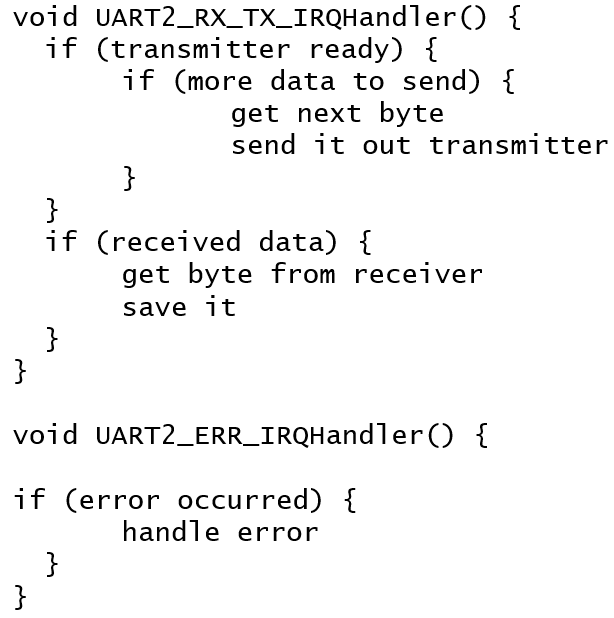
\includegraphics[scale=0.35]{09_ISRIRQ}
		\end{figure}
	\end{columns}
}
\end{frame}
%%%%%%%%%%%%%%%%% FRAME %%%%%%%%%%%%%%%%%%%%%%%%%%
\begin{frame}[fragile]
	\frametitle{Definir las colas}
	{\footnotesize
	\begin{lstlisting}[style=CStyle]
#define Q_SIZE (32)
typedef struct {
	unsigned char Data[Q_SIZE];
	unsigned int Head; // points to oldest data element
	unsigned int Tail; // points to next free space 
	unsigned int Size; // quantity of elements in queue
} Q_T;

Q_T tx_q, rx_q;

void Q_Init(Q_T *q) {
	unsigned int i;
	for (i=0; i<Q_SIZE; i++)  
		q->Data[i] = 0;  // to simplify our lives when debugging
	q->Head = 0;
	q->Tail = 0;
	q->Size = 0;
}

int Q_Empty(Q_T *q) {
	return q->Size == 0;
}
int Q_Full(Q_T *q) {
	return q->Size == Q_SIZE;
}
	\end{lstlisting}		
	}
\end{frame}
%%%%%%%%%%%%%%%%% FRAME %%%%%%%%%%%%%%%%%%%%%%%%%%
\begin{frame}[fragile]
	\frametitle{Enqueue and Dequeue}
	{\footnotesize
		\begin{lstlisting}[style=CStyle]
int Q_Enqueue(Q_T *q, unsigned char d) {
	// What if queue is full?
	if (!Q_Full(q)) {
		q->Data[q->Tail++] = d;
		q->Tail %= Q_SIZE;
		q->Size++;
		return 1; // success
	} else 
	return 0; // failure
}
unsigned char Q_Dequeue(Q_T *q) {
	// Must check to see if queue is empty before dequeueing
	unsigned char t=0;
	if (!Q_Empty(q)) {
		t = q->Data[q->Head];
		q->Data[q->Head++] = 0; // to simplify debugging
		q->Head %= Q_SIZE;
		q->Size--;
	}
	return t;
}

		\end{lstlisting}		
	}
\end{frame}

%%%%%%%%%%%%%%%%% FRAME %%%%%%%%%%%%%%%%%%%%%%%%%%
\frame{
	\begin{center}
		\vspace{3cm}
		\LARGE \textcolor{blue}{COMUNICACIONES SPI \\ (Serial Peripheral Interface)}
	\end{center}
}
%%%%%%%%%%%%%%%%% FRAME %%%%%%%%%%%%%%%%%%%%%%%%%%
\begin{frame}
	\frametitle{SPI - Arquitectura de hardware}
	
	\begin{figure}
		\centering
		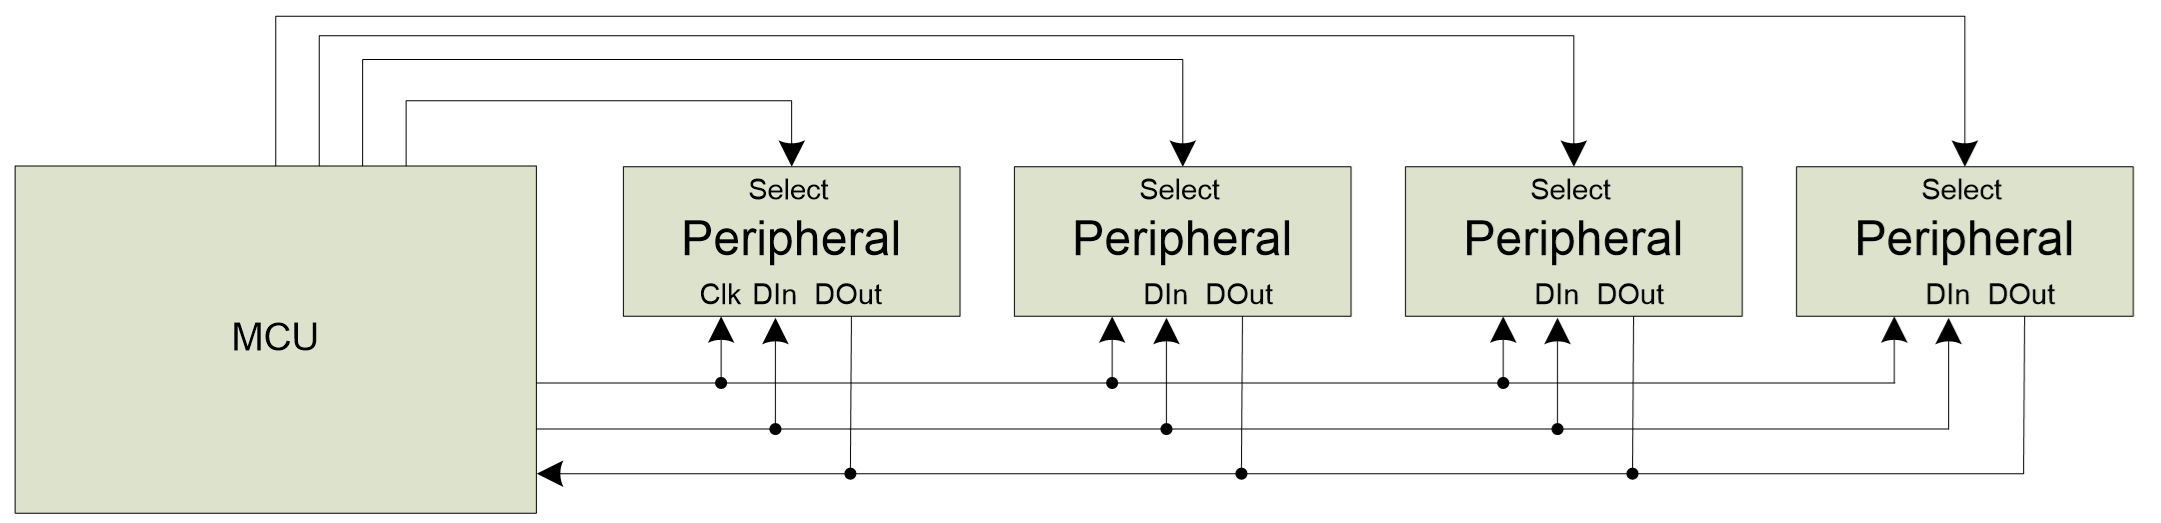
\includegraphics[scale=0.35]{10_SPIArchitecture}
	\end{figure}
	
	\begin{itemize}
		\item Todos los chips comparten el bus de señales.
		\begin{itemize}
			\item Clock SCK
			\item Líneas de datos: MOSI (master out, slave in) y MISO (master in, slave out)
		\end{itemize}
		\item Cada periférico tiene su propio selector (chip select CS)
		\begin{itemize}
			\item El maestro activa la línea CS solo con el periférico que se está comunicando. 
		\end{itemize}
	\end{itemize}
\end{frame}
%%%%%%%%%%%%%%%%% FRAME %%%%%%%%%%%%%%%%%%%%%%%%%%
\begin{frame}
	\frametitle{SPI - Transmisión serial}
	
	\begin{figure}
		\centering
		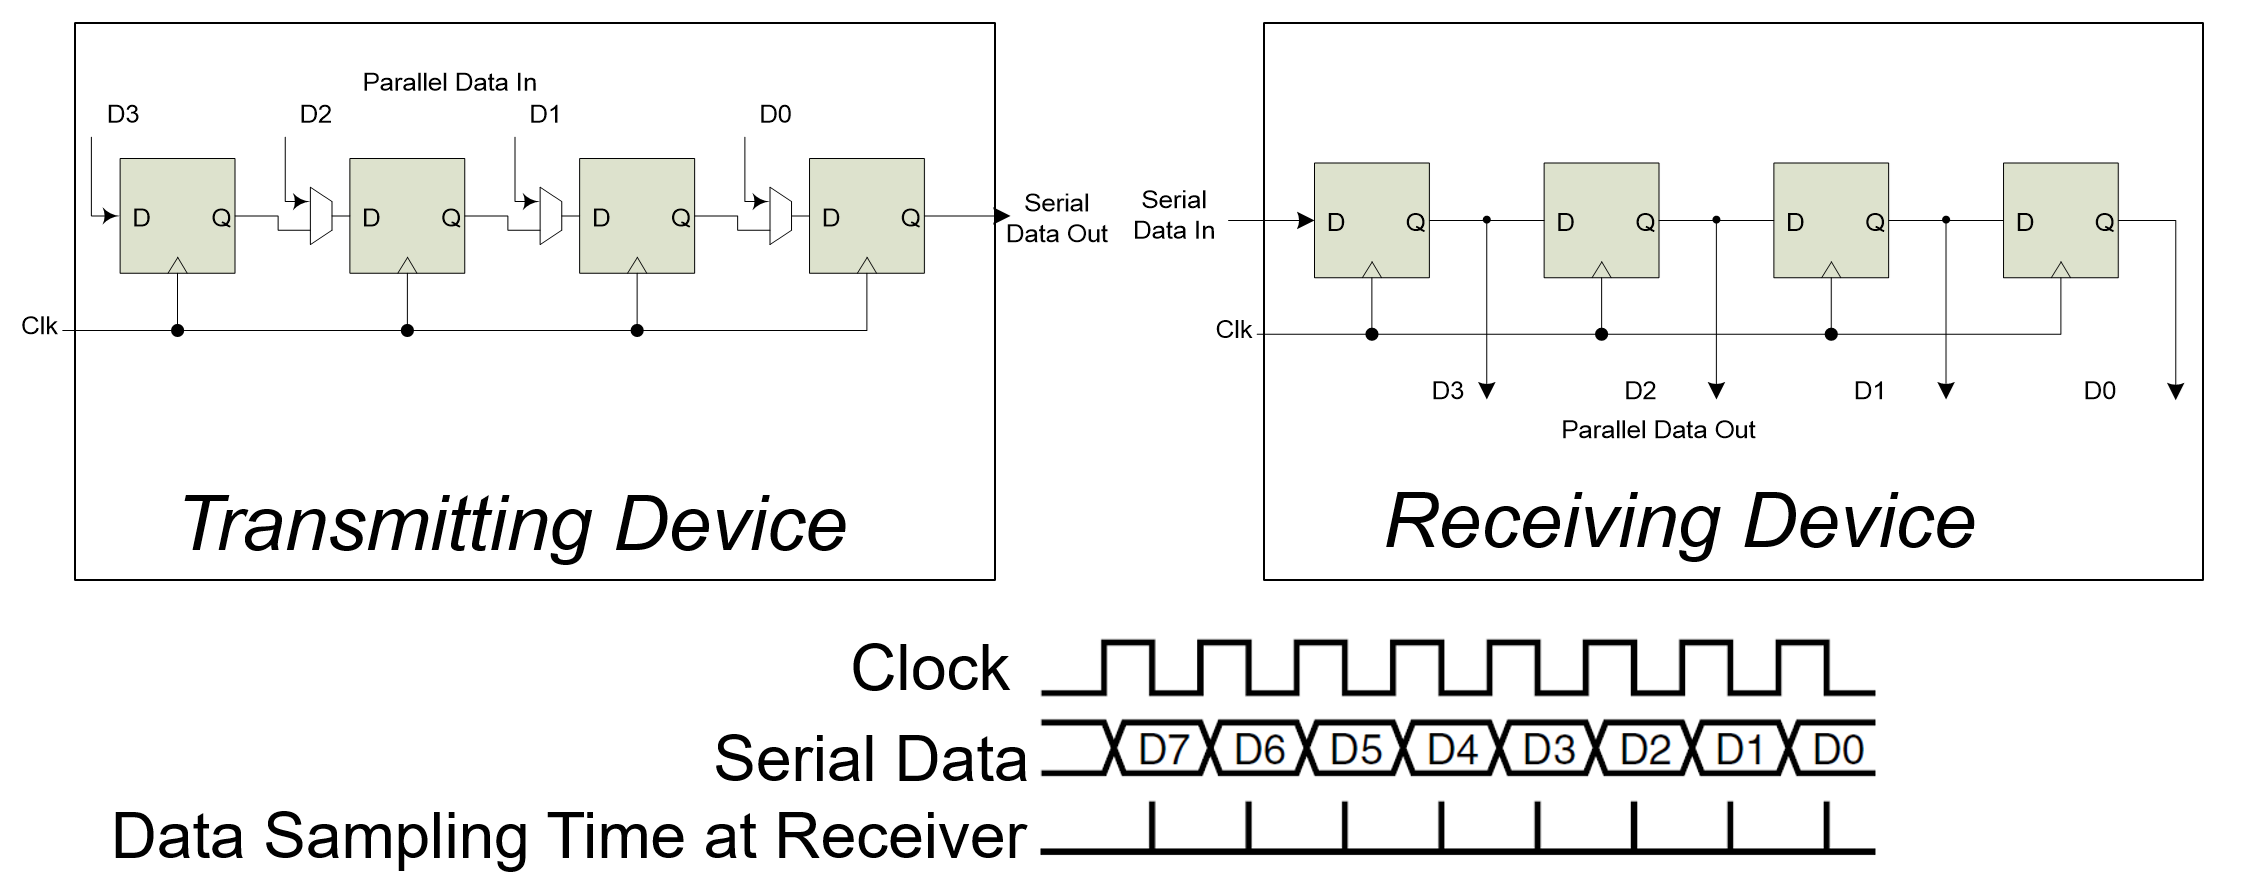
\includegraphics[scale=0.35]{11_SPISerial}
	\end{figure}
	
	\begin{itemize}
		\item Utiliza shift register y señales de clock para convertir entre serial y paralelo.
		\item \textbf{Sincrónico}: una señal de clock explícita va en conjunto con las líneas de datos. 
	\end{itemize}
\end{frame}
%%%%%%%%%%%%%%%%% FRAME %%%%%%%%%%%%%%%%%%%%%%%%%%
\begin{frame}
	\frametitle{SPI - Diagrama y registros}
	
	\begin{figure}
		\centering
		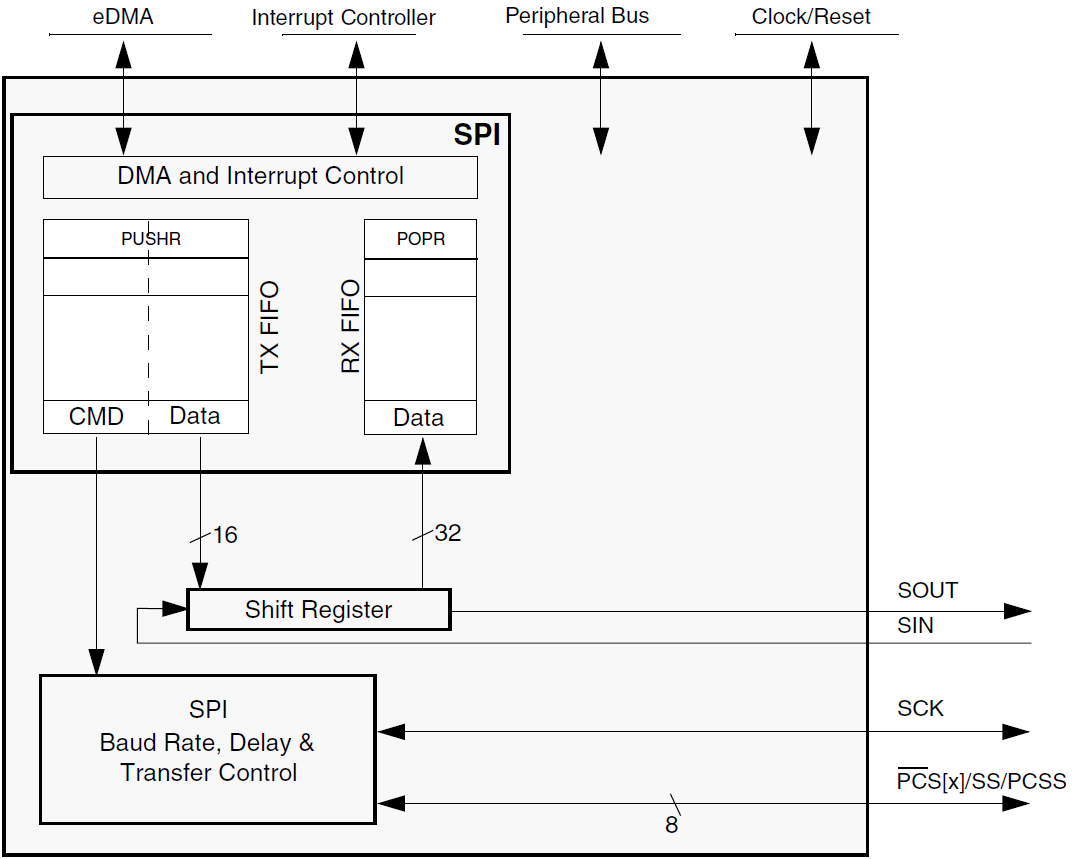
\includegraphics[scale=0.3]{12_SPIDiagram}
	\end{figure}
	
	\begin{itemize}
		\item La comunicación SPI consiste en intercambiar datos entre el maestro y el esclavo. Al mismo tiempo se desplaza el de envió como el de recepción.
		\item El MCU K64F cuenta con tres SPI, los cuales a su vez cuentan con pilas para la transmisión y recepción de datos. 
		\begin{itemize}
			\item SPI0: 4 FIFO para Tx y Rx, SPI1 y SPI2: 1 FIFO para Tx y Rx
		\end{itemize}
	\end{itemize}
\end{frame}
%%%%%%%%%%%%%%%%% FRAME %%%%%%%%%%%%%%%%%%%%%%%%%%
\begin{frame}
	\frametitle{SPI - Registros}
	{\small
	\textcolor{blue}{Module Configuration Register - SPI0\_MCR}
	
	\begin{columns}
		\column{0.4\linewidth}
		\begin{figure}
			\centering
			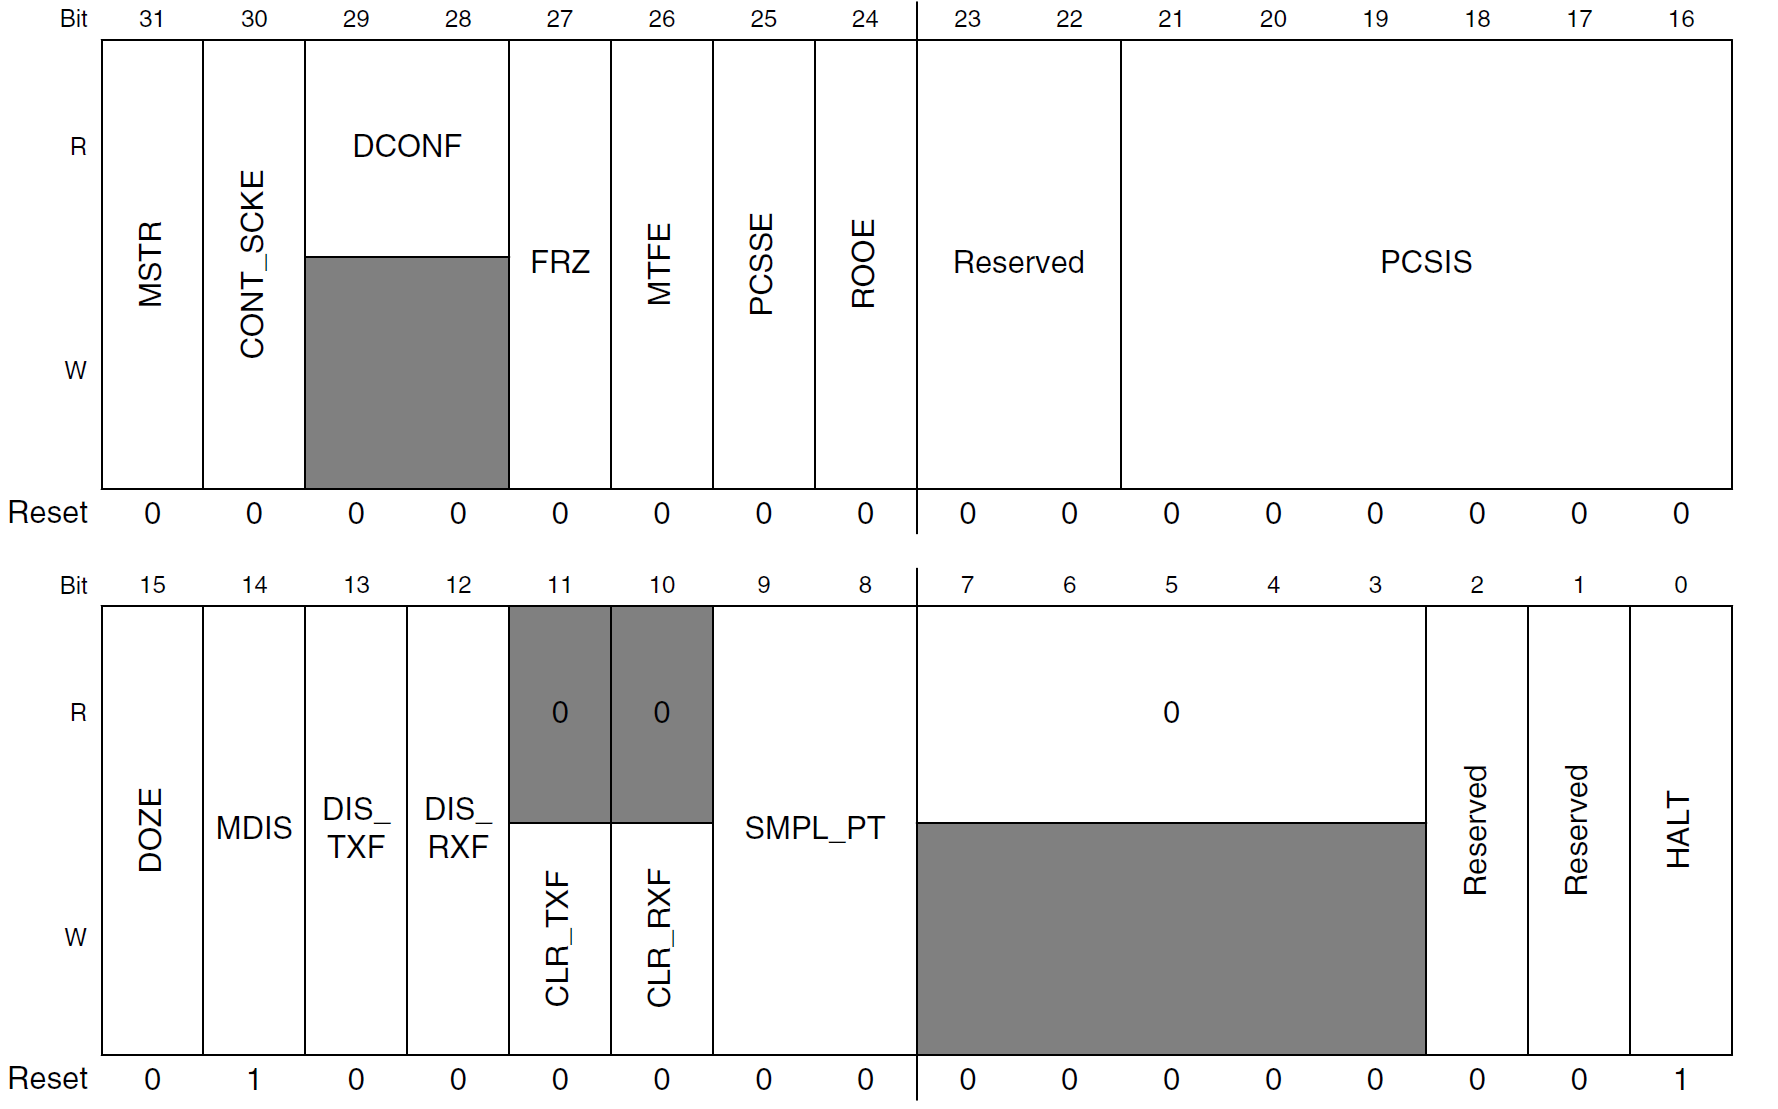
\includegraphics[scale=0.2]{13_SPIMCR}
		\end{figure}
	
		\column{0.6\linewidth}
		\begin{itemize}
			\item MSTR: 1 modo maestro, 0 modo esclavo.
			\item FRZ: detiene la transferencia serial en modo config.
			\item PCSIS: el estado inactivo del chip select
			\item MDIS: habilitar o deshabilitar el módulo
			\item DIS\_TXF: deshabilitar el Tx FIFO
			\item DIS\_RXF: deshabilitar el Rx FIFO
			\item HALT: Para las transferencias
		\end{itemize}
	\end{columns}
	}
\end{frame}
%%%%%%%%%%%%%%%%% FRAME %%%%%%%%%%%%%%%%%%%%%%%%%%
\begin{frame}
	\frametitle{SPI - Registros}
	{\small
		\textcolor{blue}{Clock y atributos de transferencia - SPI0\_CTAR}
		
		\begin{columns}
			\column{0.4\linewidth}
			\begin{figure}
				\centering
				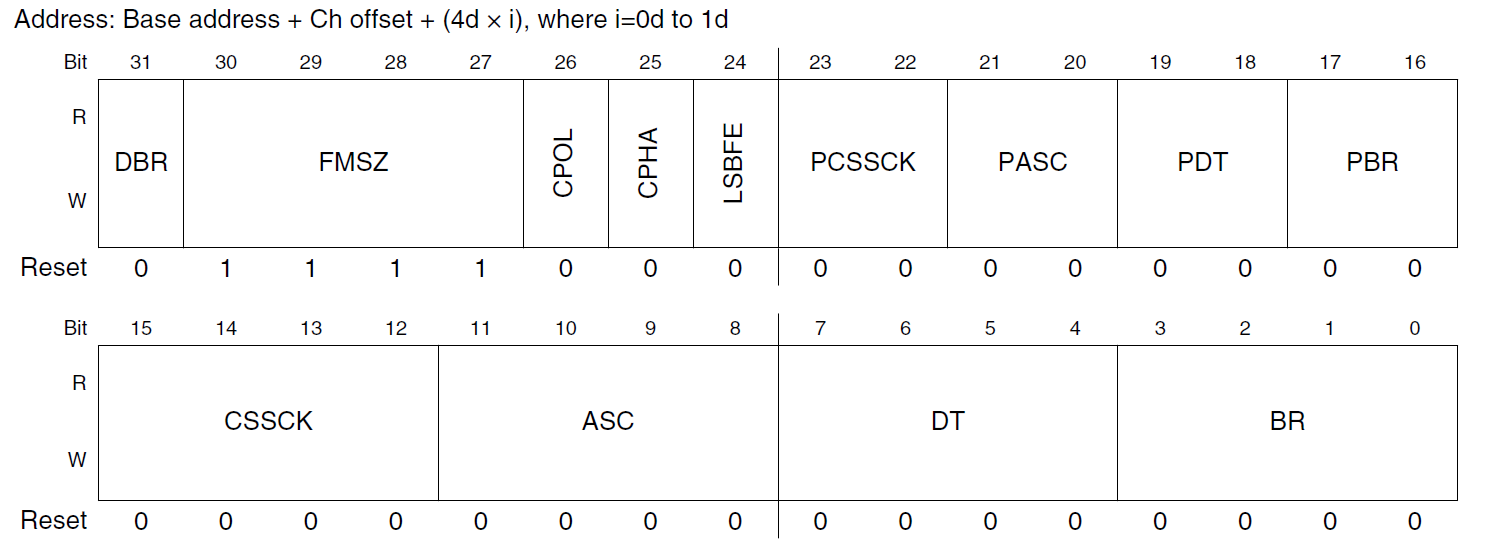
\includegraphics[scale=0.25]{14_SPICTAR}
			\end{figure}
			
			\column{0.6\linewidth}
			\begin{itemize}
				\item DBR: dobla el baud rate.
				\item FMSZ: el número de bits a enviar más uno. El mínimo es 4.
				\item CPOL: polaridad del clock
				\item CPHA: fase del clock
				\item LSBFE: primero se transmite el menos significativo
				\item PBR: Baud rate preescaler.
				\item BR: Baud rate escaler.
			\end{itemize}
		\end{columns}
	}
\end{frame}
%%%%%%%%%%%%%%%%% FRAME %%%%%%%%%%%%%%%%%%%%%%%%%%
\begin{frame}
	\frametitle{SPI - Modos}
	{\small
	
		\begin{columns}
			\column{0.4\linewidth}
			\begin{figure}
				\centering
				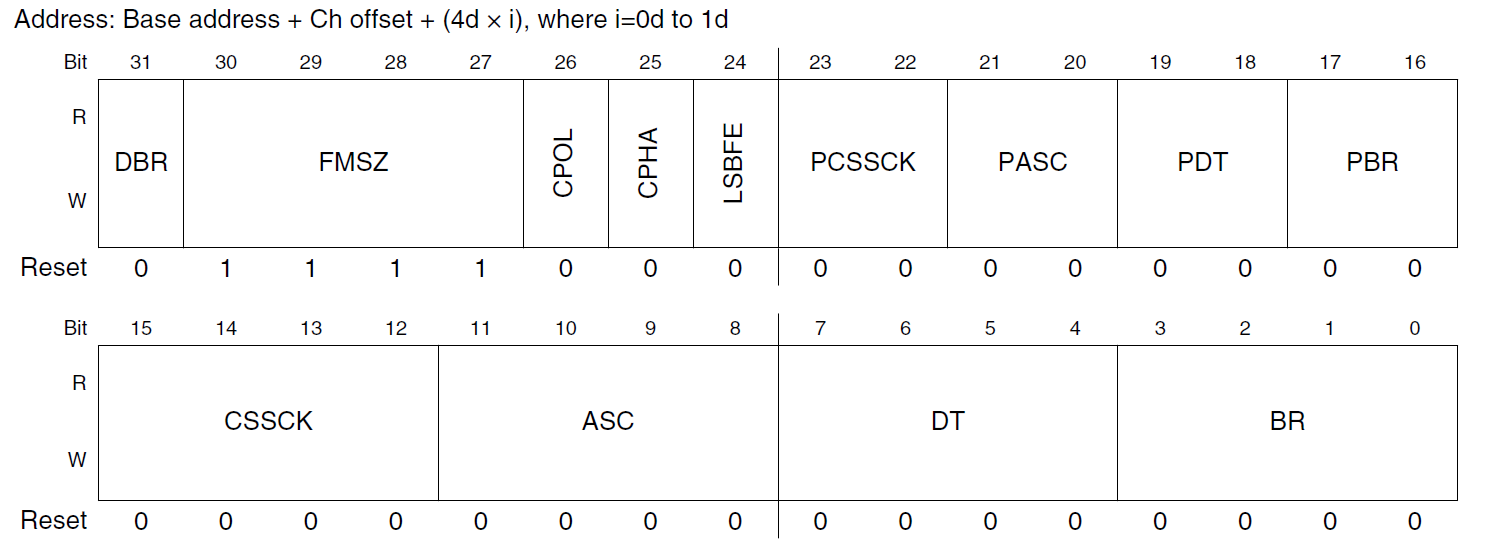
\includegraphics[scale=0.25]{14_SPICTAR}
			\end{figure}
			
			\column{0.6\linewidth}
			\begin{itemize}
				\item DBR: dobla el baud rate.
				\item FMSZ: el número de bits a enviar más uno. El mínimo es 4.
				\item CPOL: polaridad del clock
				\item CPHA: fase del clock
				\item LSBFE: primero se transmite el menos significativo
				\item PBR: Baud rate preescaler.
				\item BR: Baud rate escaler.
			\end{itemize}
		\end{columns}
	}
\end{frame}
%%%%%%%%%%%%%%%%% FRAME %%%%%%%%%%%%%%%%%%%%%%%%%%
\begin{frame}
	\frametitle{SPI - Registros}
	{\small
			\begin{figure}
				\centering
				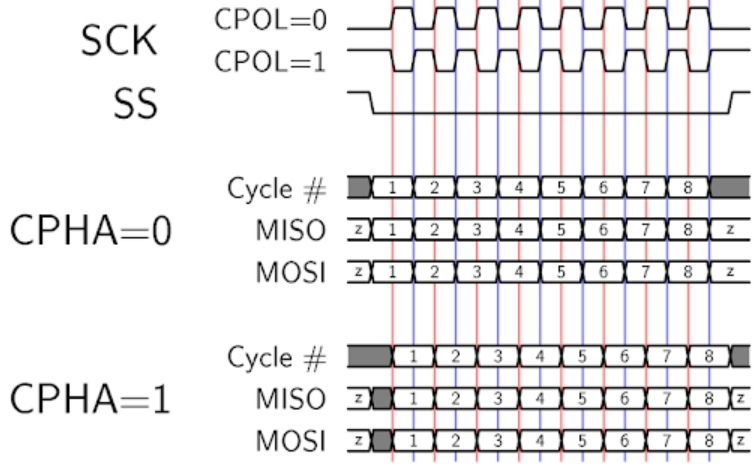
\includegraphics[scale=0.9]{16_SPIModos}
			\end{figure}		
	}
\end{frame}
%%%%%%%%%%%%%%%%% FRAME %%%%%%%%%%%%%%%%%%%%%%%%%%
\begin{frame}
	\frametitle{SPI - Ejemplo}
	{\small
		Se requiere leer un termopar tipo k el cual esta conectado a través de un transmisor MAX6675 con salida o protocolo SPI
		
		\textbf{Solución}: 
		
		\begin{itemize}
			\item Revisar la hoja de datos del \href{https://datasheets.maximintegrated.com/en/ds/MAX6675.pdf}{MAX 6675}.
			\item Inicializar el clock del bus
			\item Inicializar los clocks y puertos del SPI.
			\item Inicializar los registros PCR para que los pines trabajen en modo SPI
			\item Configurar el SPI
		\end{itemize}
	}
\end{frame}

%%%%%%%%%%%%%%%%% FRAME %%%%%%%%%%%%%%%%%%%%%%%%%%
\begin{frame}
	\frametitle{SPI - Ejemplo}
	{\small
		\begin{columns}
			\column{0.4\linewidth}
			\begin{figure}
				\centering
				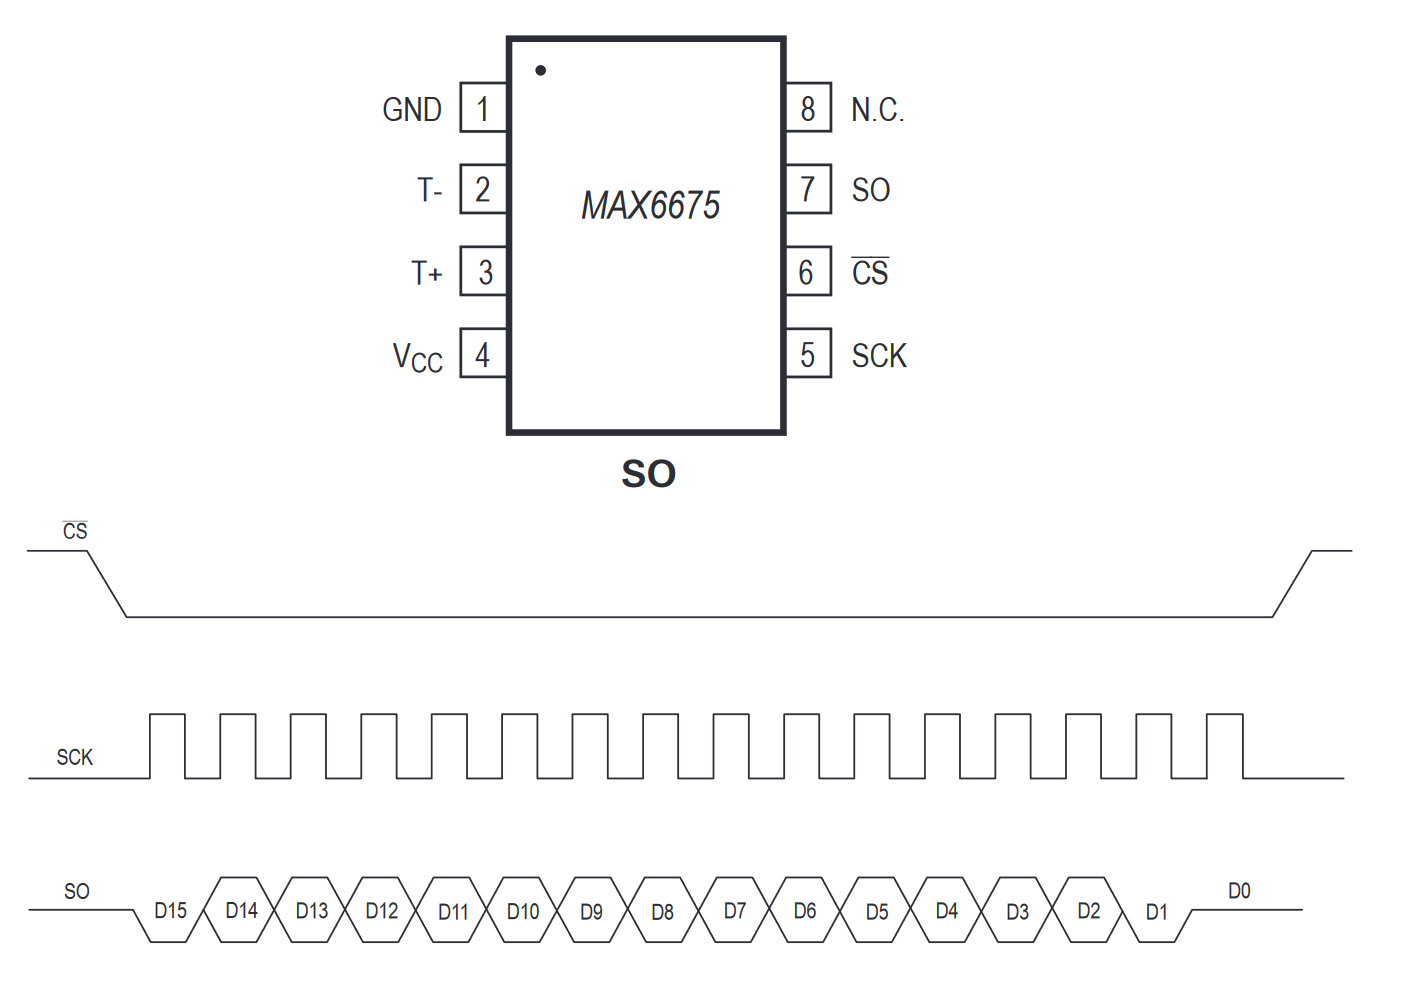
\includegraphics[scale=0.25]{17_EjemploSPI}
			\end{figure}
			
			\column{0.6\linewidth}
			\begin{itemize}
				\item Solo se requiere conectar la línea de datos MISO, no MOSI.
				\item El dataframe es de 16 bits. El dato se encuentra entre D14-D3 del más significativo al menos. 
				\item D2 esta en alto cuando no está el termopar
				\item D1 está en bajo, y D0 tres estados. 
				\item Los datos se capturan en flanco de bajada
				\item Todo cero corresponde a \SI{0}{\degreeCelsius} y todos unos a \SI{1023}{\degreeCelsius}. 
				\item Máxima velocidad del clock \SI{4.3}{\mega\hertz}
			\end{itemize}
		\end{columns}
	}
\end{frame}
%%%%%%%%%%%%%%%%% FRAME %%%%%%%%%%%%%%%%%%%%%%%%%%
\begin{frame}[fragile]
	\frametitle{SPI - Ejemplo}
	{\small
		
	Configuración del SPI
		
		\begin{lstlisting}[style=CStyle]
void Init_SPI0(void){
	// Enable clock to SPI0 and PORTD
	SIM->SCGC5 |= SIM_SCGC5_PORTD_MASK;
	SIM->SCGC6 |= SIM_SCGC6_SPI0_MASK;
	
	// Enable SPI and stops transfers SPI in debug mode
	SPI0->MCR &= ~SPI_MCR_MDIS_MASK;
	SPI0->MCR |= SPI_MCR_HALT_MASK;
	
	// Set PTD0 as SPI0_PCS0 -- ALT2
	PORTD->PCR[0] &= ~PORT_PCR_MUX_MASK;
	PORTD->PCR[0] |= PORT_PCR_MUX(2);
	
	// Set PTD1 as SPI0_SCK -- ALT2
	PORTD->PCR[1] &= ~PORT_PCR_MUX_MASK;
	PORTD->PCR[1] |= PORT_PCR_MUX(2);
	
	// Set PTD2 as SPI0_SOUT -- ALT2
	PORTD->PCR[2] &= ~PORT_PCR_MUX_MASK;
	PORTD->PCR[2] |= PORT_PCR_MUX(2);
	
	// Set PTD3 as SPI0_SIN -- ALT2
	PORTD->PCR[3] &= ~PORT_PCR_MUX_MASK;
	PORTD->PCR[3] |= PORT_PCR_MUX(2);
		\end{lstlisting}	
	}
\end{frame}
%%%%%%%%%%%%%%%%% FRAME %%%%%%%%%%%%%%%%%%%%%%%%%%
\begin{frame}[fragile]
	\frametitle{SPI - Ejemplo}
	{\tiny
		\begin{lstlisting}[style=CStyle]
	// Enable master mode, inactive SS is high
	SPI0->MCR |= SPI_MCR_MSTR_MASK | SPI_MCR_PCSIS_MASK;
	
	// SCK baud rate = (Bus Clock /PBR) x [(1+DBR)/BR]
	// SCK = (60MHz/7) x [1/8192] = 1 kHz approx 1.046 kHz
	uint32_t temp;
	temp = SPI0->CTAR[0] & ~(SPI_CTAR_DBR_MASK | SPI_CTAR_PBR_MASK | SPI_CTAR_BR_MASK);
	SPI0->CTAR[0] = temp | SPI_CTAR_DBR(0)|
					SPI_CTAR_PBR(3)|
					SPI_CTAR_BR(12);
	
	// Temp variable with zeros in changed fields
	temp = SPI0->CTAR[0] &~(SPI_CTAR_FMSZ_MASK | SPI_CTAR_CPOL_MASK | SPI_CTAR_CPHA_MASK | SPI_CTAR_LSBFE_MASK);
	
	// Dataframe de 16 bits, inactive SCK is low, CPHA is one where data is changed on the leading edge, MSB first
	SPI0->CTAR[0] = temp | SPI_CTAR_FMSZ(16-1) |
					SPI_CTAR_CPOL(1) |
					SPI_CTAR_CPHA(1) |
					SPI_CTAR_LSBFE(0);
	
	// Enable SPI transfer
	SPI0->MCR &= ~SPI_MCR_HALT_MASK;
}
			
		\end{lstlisting}	
	}
\end{frame}
%%%%%%%%%%%%%%%%% FRAME %%%%%%%%%%%%%%%%%%%%%%%%%%
\begin{frame}[fragile]
	\frametitle{SPI - Ejemplo}
	{\small
		Envió y recepción de datos. 
		
		\begin{lstlisting}[style=CStyle]
uint32_t SPI_send(uint16_t data){
	uint32_t dataRx;
	
	// Push data to Tx FIFO, and PCS = 0
	SPI0->PUSHR = (SPI_PUSHR_PCS(1) | data);
	// Wait for Tx buffer empty
	while(!(SPI0->SR & SPI_SR_TCF_MASK));
	SPI0->SR |= SPI_SR_TCF_MASK;
	
	
	// Wait for data in Rx buffer
	while (!(SPI0->SR & SPI_SR_RFDF_MASK));
	//Read data
	dataRx = SPI0->POPR;
	SPI0->SR |= SPI_SR_RFDF_MASK;
	return dataRx;
	
}
		
	\end{lstlisting}	
}
\end{frame}

%%%%%%%%%%%%%%%%% FRAME %%%%%%%%%%%%%%%%%%%%%%%%%%
\begin{frame}[fragile]
	\frametitle{SPI - Ejemplo}
	{\small
		Main. 
		
		\begin{lstlisting}[style=CStyle]
int main(void) {
	float temperature = 0;
	
	/* Init board hardware. */
	BOARD_InitBootClocks();
	Init_SPI0();
	
	while(1) {
		temperature = ((float)(SPI_send(0x00)>>3))/4.0;
	}
	return 0 ;
}
			
		\end{lstlisting}	
	}
\end{frame}

%%%%%%%%%%%%%%%%% FRAME %%%%%%%%%%%%%%%%%%%%%%%%%%
\begin{frame}
	\frametitle{SPI - Ejemplo 2}
	{\small
		Utilice el SDK para resolver el mismo problema. 
		
		Solución:
		
		\begin{itemize}
			\item Configure el reloj del sistema. Recuerde que muchos periféricos trabajan es con el clock del Bus.
			\item Habilite los puertos o pines a trabajar. Recuerde que esto implica activar el clock y ponerlos en la alternativa a trabajar
			\item Configure los periféricos que vaya a usar.
			\item Utilice el API de los drivers de cada periférico. 
		\end{itemize}	
	}
\end{frame}
%%%%%%%%%%%%%%%%% FRAME %%%%%%%%%%%%%%%%%%%%%%%%%%
\begin{frame}
	\frametitle{SPI - Ejemplo 2}
	\begin{figure}
		\centering
		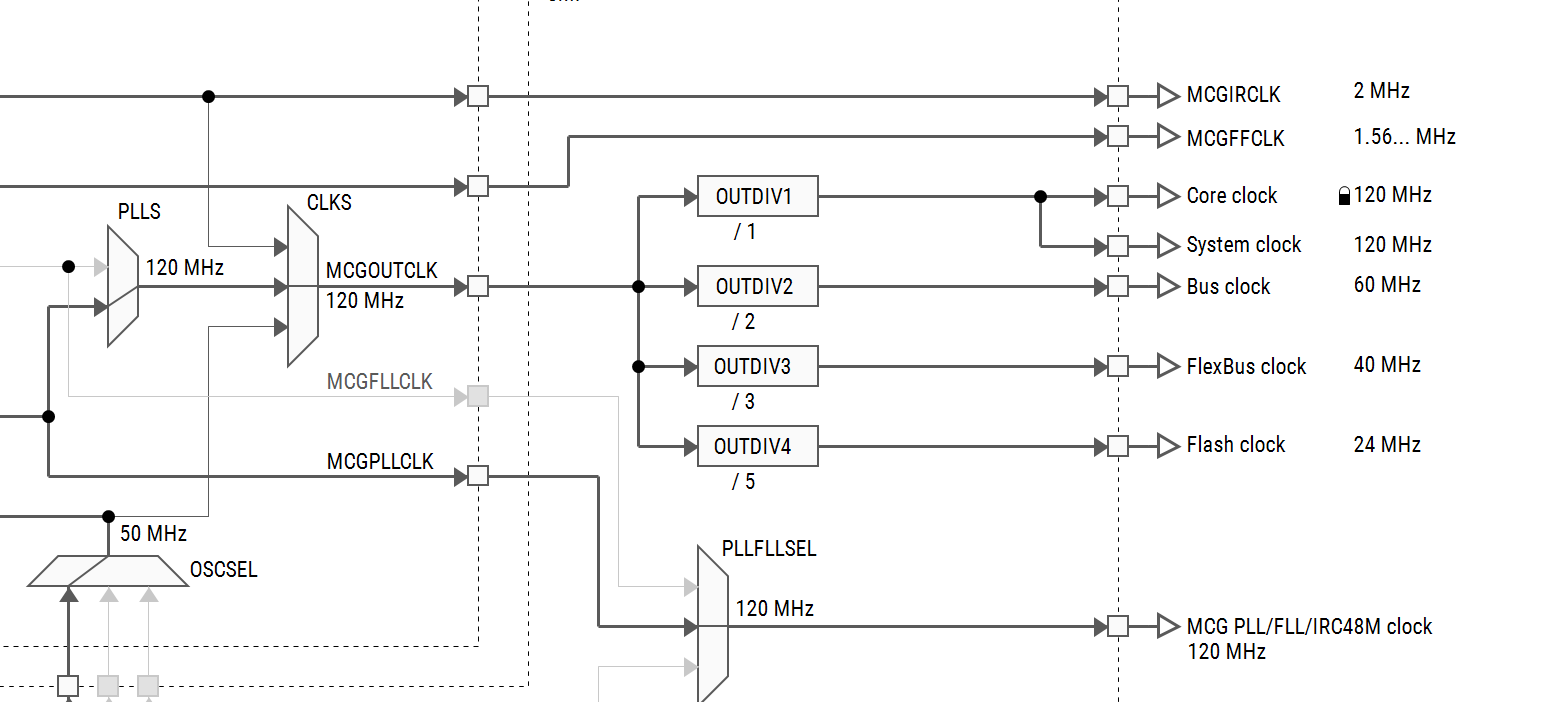
\includegraphics[scale=0.5]{19_ClockConfig}
	\end{figure}
\end{frame}
%%%%%%%%%%%%%%%%% FRAME %%%%%%%%%%%%%%%%%%%%%%%%%%
\begin{frame}
	\frametitle{SPI - Ejemplo 2}
	\begin{figure}
		\centering
		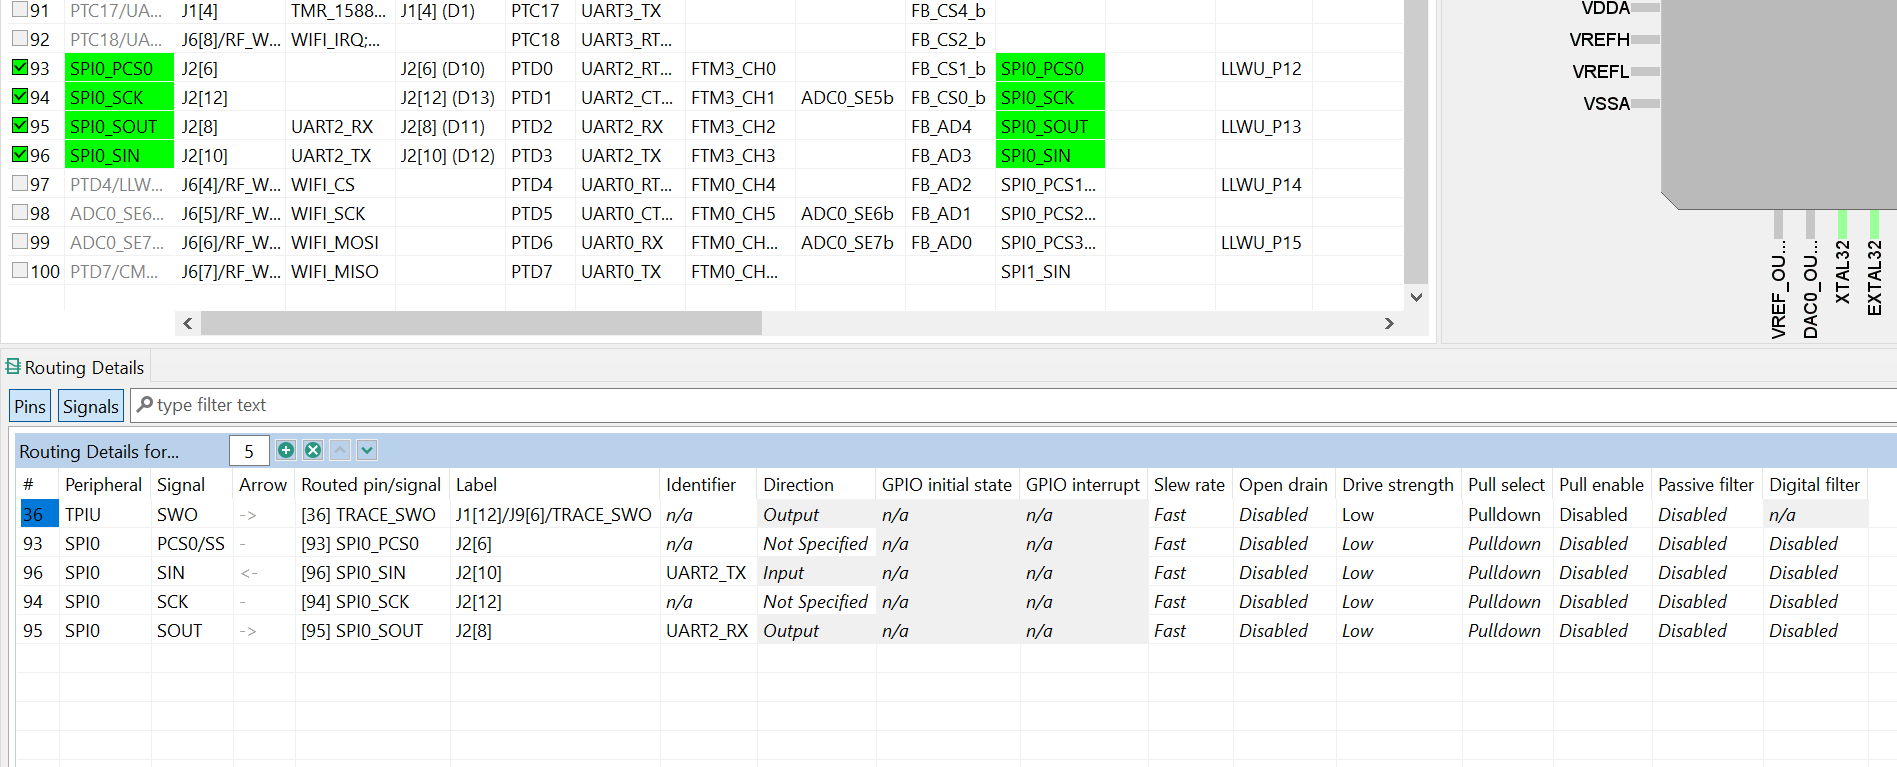
\includegraphics[scale=0.4]{18_SPIPinActivate}
	\end{figure}
\end{frame}
%%%%%%%%%%%%%%%%% FRAME %%%%%%%%%%%%%%%%%%%%%%%%%%
\begin{frame}
	\frametitle{SPI - Ejemplo 2}
	\begin{figure}
		\centering
		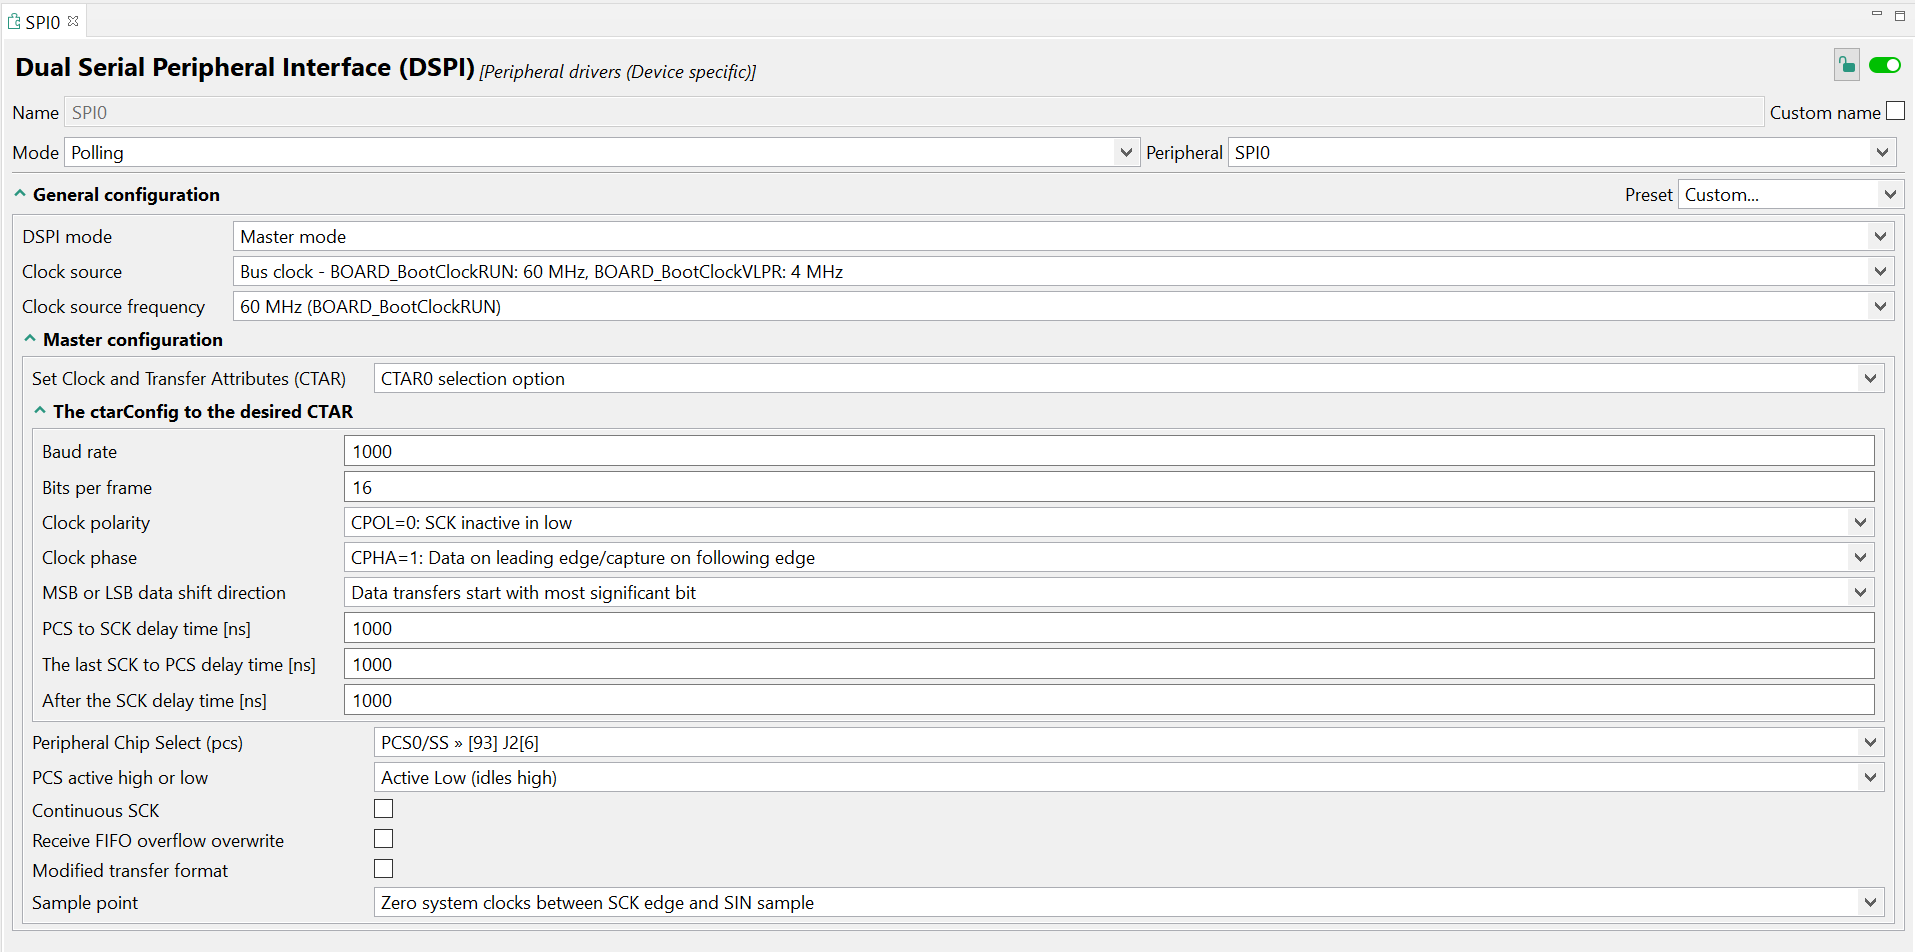
\includegraphics[scale=0.4]{20_SPI0Config}
	\end{figure}
\end{frame}
%%%%%%%%%%%%%%%%% FRAME %%%%%%%%%%%%%%%%%%%%%%%%%%
\begin{frame}[fragile]
	\frametitle{SPI - Ejemplo 2}
	\begin{lstlisting}[style=CStyle]
int main(void) {
	
	float temperature;
	
	/* Init board hardware. */
	BOARD_InitBootPins();
	BOARD_InitBootClocks();
	BOARD_InitBootPeripherals();
	#ifndef BOARD_INIT_DEBUG_CONSOLE_PERIPHERAL
	/* Init FSL debug console. */
	BOARD_InitDebugConsole();
	#endif
	
	// Command configuration for SPI
	dspi_command_data_config_t SPI0Config;
	SPI0Config.isPcsContinuous=false;
	SPI0Config.whichCtar = kDSPI_Ctar0;
	SPI0Config.whichPcs = kDSPI_Pcs0;
	SPI0Config.clearTransferCount = false;
	SPI0Config.isEndOfQueue = false;
	
	while(1) {
		DSPI_MasterWriteDataBlocking(SPI0, \&SPI0Config, 0x00);
		uint32_t DataSPI = DSPI_ReadData(SPI0);
		temperature = ((float)(DataSPI>>3))/4.0;
		PRINTF("La temperatura es: %f\n\r",temperature);
	}
	return 0 ;
}
	
	
	\end{lstlisting}
\end{frame}

%%%%%%%%%%%%%%%%% FRAME %%%%%%%%%%%%%%%%%%%%%%%%%%
\frame{
	\begin{center}
		\vspace{3cm}
		\LARGE \textcolor{blue}{COMUNICACIONES I2C \\ (Inter-Integrated Circuit)}
	\end{center}
}

%%%%%%%%%%%%%%%%% FRAME %%%%%%%%%%%%%%%%%%%%%%%%%%
\begin{frame}
	\frametitle{I2C - Conceptos}
	{\small
		
		\begin{columns}
			\column{0.5\linewidth}
			\begin{itemize}
				\item Múltiples dispositivos conectados al mismo bus serial.
				\item El bus es controlador por un dispositivo maestro, y los esclavos responden cuando se envían sus direcciones. 
				\item El bus I2C tiene dos señales: SDA y SCL.
				\item Todos los detalles se encuentra en su protocolo de definición. 
			\end{itemize}
			
			
			\column{0.5\linewidth}
			\begin{figure}
				\centering
				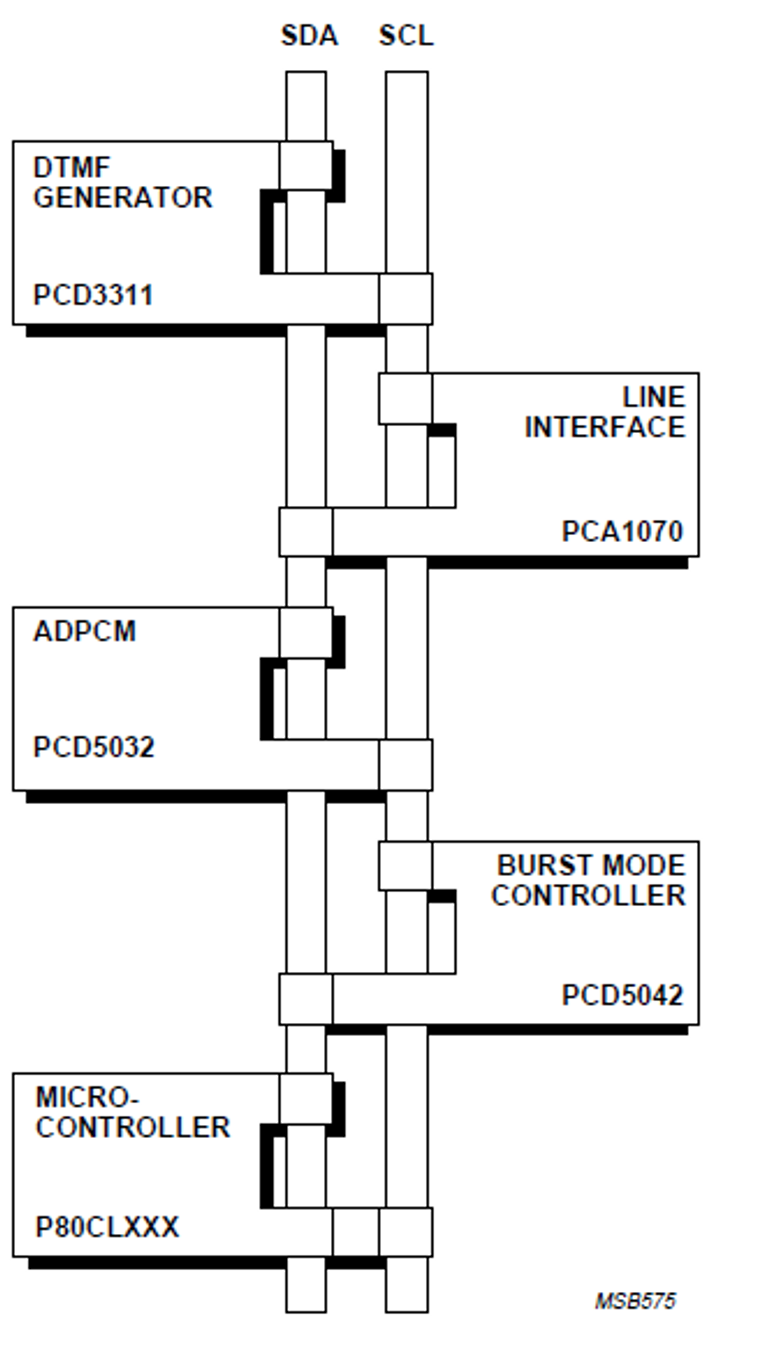
\includegraphics[scale=0.25]{21_I2CBus}
			\end{figure}
			
		\end{columns}
	}
\end{frame}
%%%%%%%%%%%%%%%%% FRAME %%%%%%%%%%%%%%%%%%%%%%%%%%
\begin{frame}
	\frametitle{I2C - Conceptos}
	{\small
		\begin{figure}
			\centering
			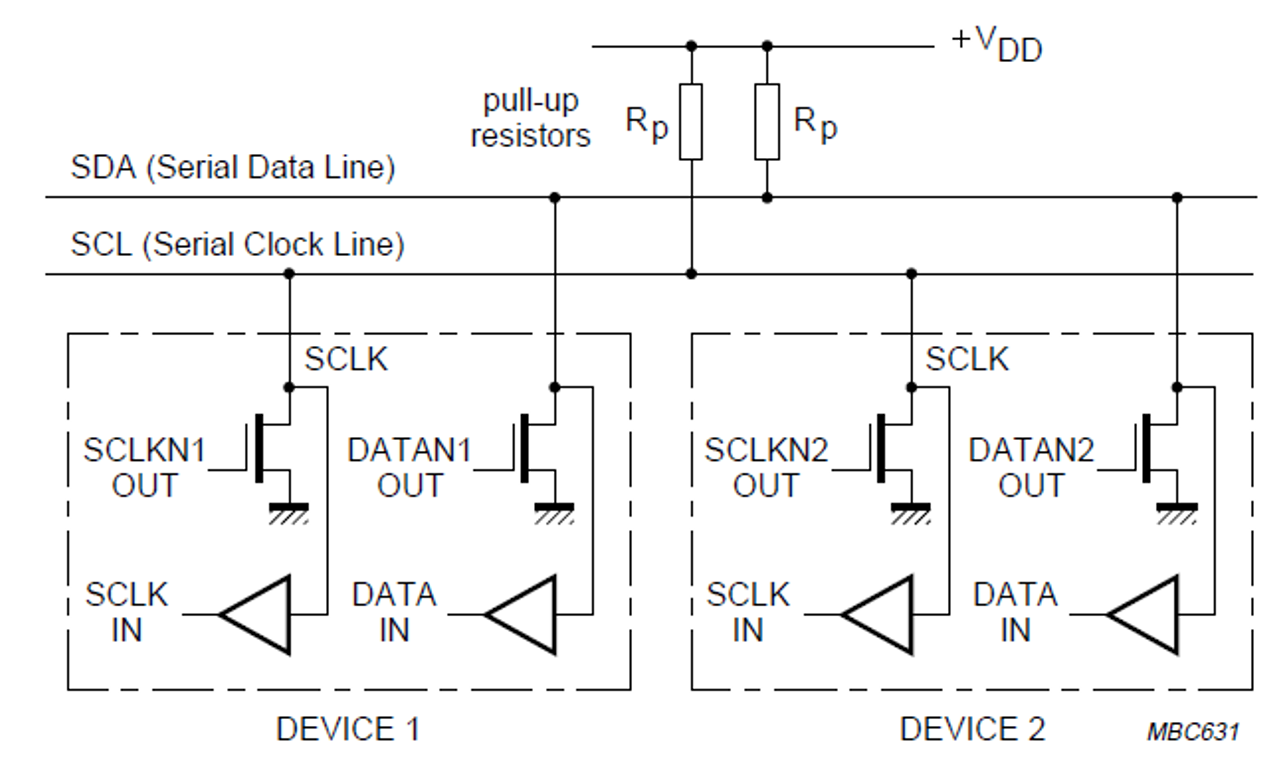
\includegraphics[scale=0.4]{22_I2CBus2}
		\end{figure}
		\begin{itemize}
			\item Resistencia de pull-up a Vdd.
			\item Transistores en drenaje abierto llevan la linea a tierra
			\item El maestro genera la señal de clock que se distribuye a todos. Puede estar entre los rangos de \SI{400}{\kilo\hertz}, \SI{1}{\mega\hertz} o más. 
		\end{itemize}
	}
\end{frame}
%%%%%%%%%%%%%%%%% FRAME %%%%%%%%%%%%%%%%%%%%%%%%%%
\begin{frame}
	\frametitle{I2C - Formato de comunicación}
	{\small
		\begin{figure}
			\centering
			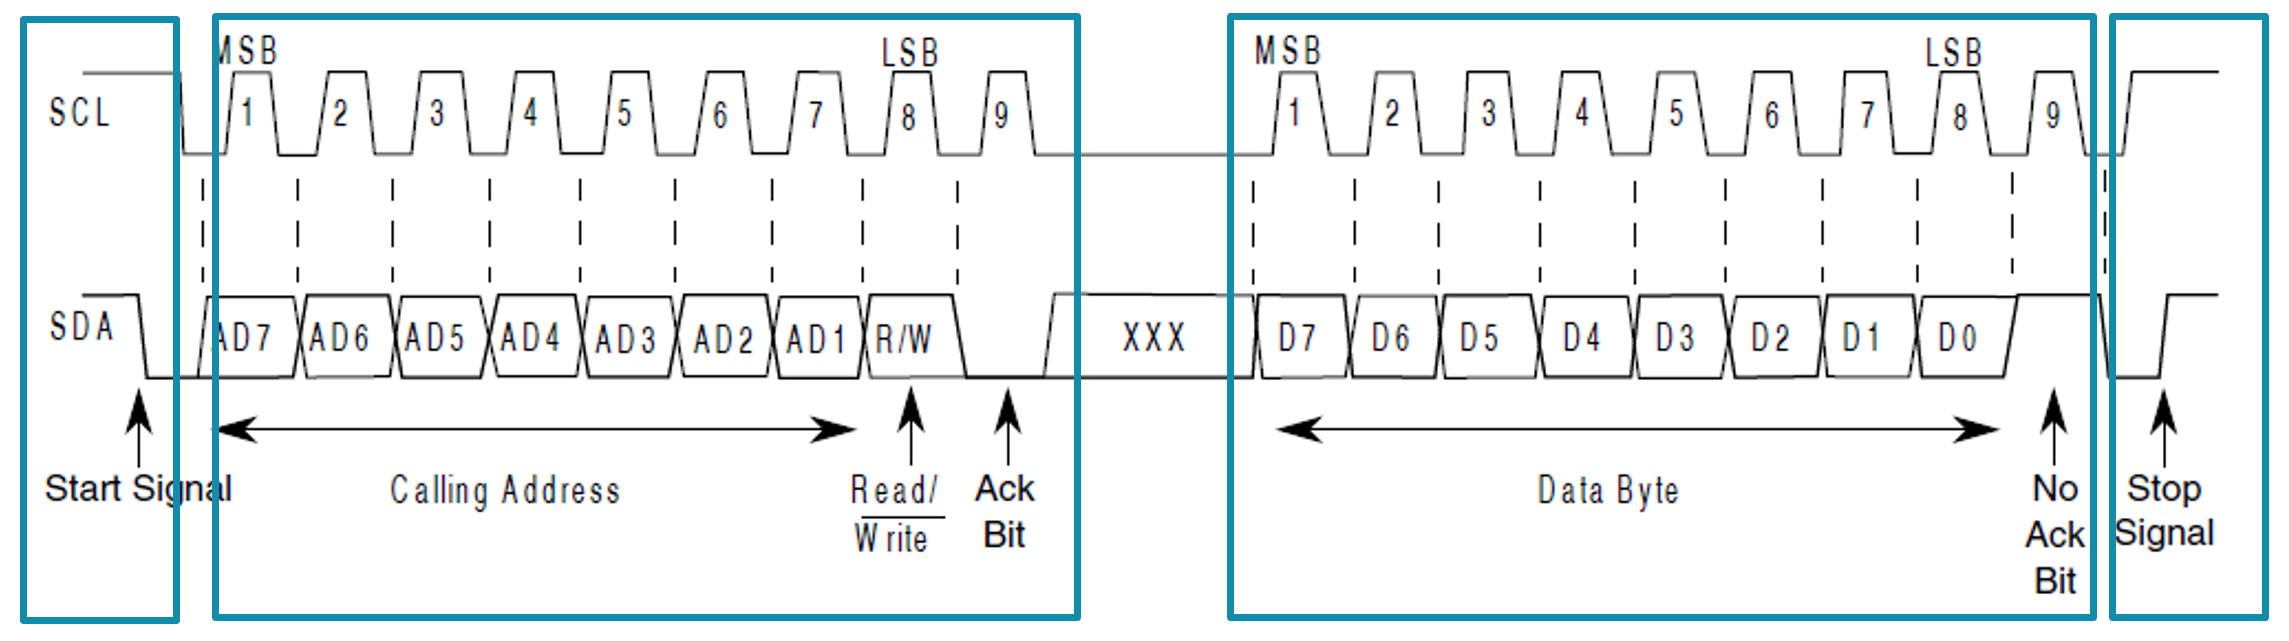
\includegraphics[scale=0.3]{23_I2CFormat}
		\end{figure}
		\begin{itemize}
			\item Transferencia de datos orientado a los mensajes con cuatro partes
			\begin{itemize}
				\item Condición de start
				\item Transmisión de la dirección del esclavo
				\begin{itemize}
					\item Dirección
					\item Escritura o Lectura
					\item ACK por parte del receptor
				\end{itemize}
				\item Campo de datos: byte de datos y ACK
				\item Condición de stop
			\end{itemize}
		\end{itemize}
	}
\end{frame}
%%%%%%%%%%%%%%%%% FRAME %%%%%%%%%%%%%%%%%%%%%%%%%%
\begin{frame}
	\frametitle{I2C - Direccionamiento}
	{\small
	\begin{columns}
		\column{0.5\linewidth}
		\begin{itemize}
			\item Direccionamiento a esclavo
			\begin{itemize}
				\item Cada esclavo tiene 7 bits de direccionamiento.
				\item Puede soportar hasta 128 dispositivos
				\item Diferentes dipositivos deben tener diferentes direcciones por defecto
				\item A veces se puede seleccionar una segunda dirección. 
			\end{itemize}
			\item Direccionamiento a registro
			\begin{itemize}
				\item Algunos dispositivos tiene señales de control, registros de datos, o memoria, como se accede a esta?
				\item Usa el primer byte de datos como direccionamiento a registro
			\end{itemize} 
		\end{itemize}
		
		
		\column{0.5\linewidth}
		\begin{figure}
			\centering
			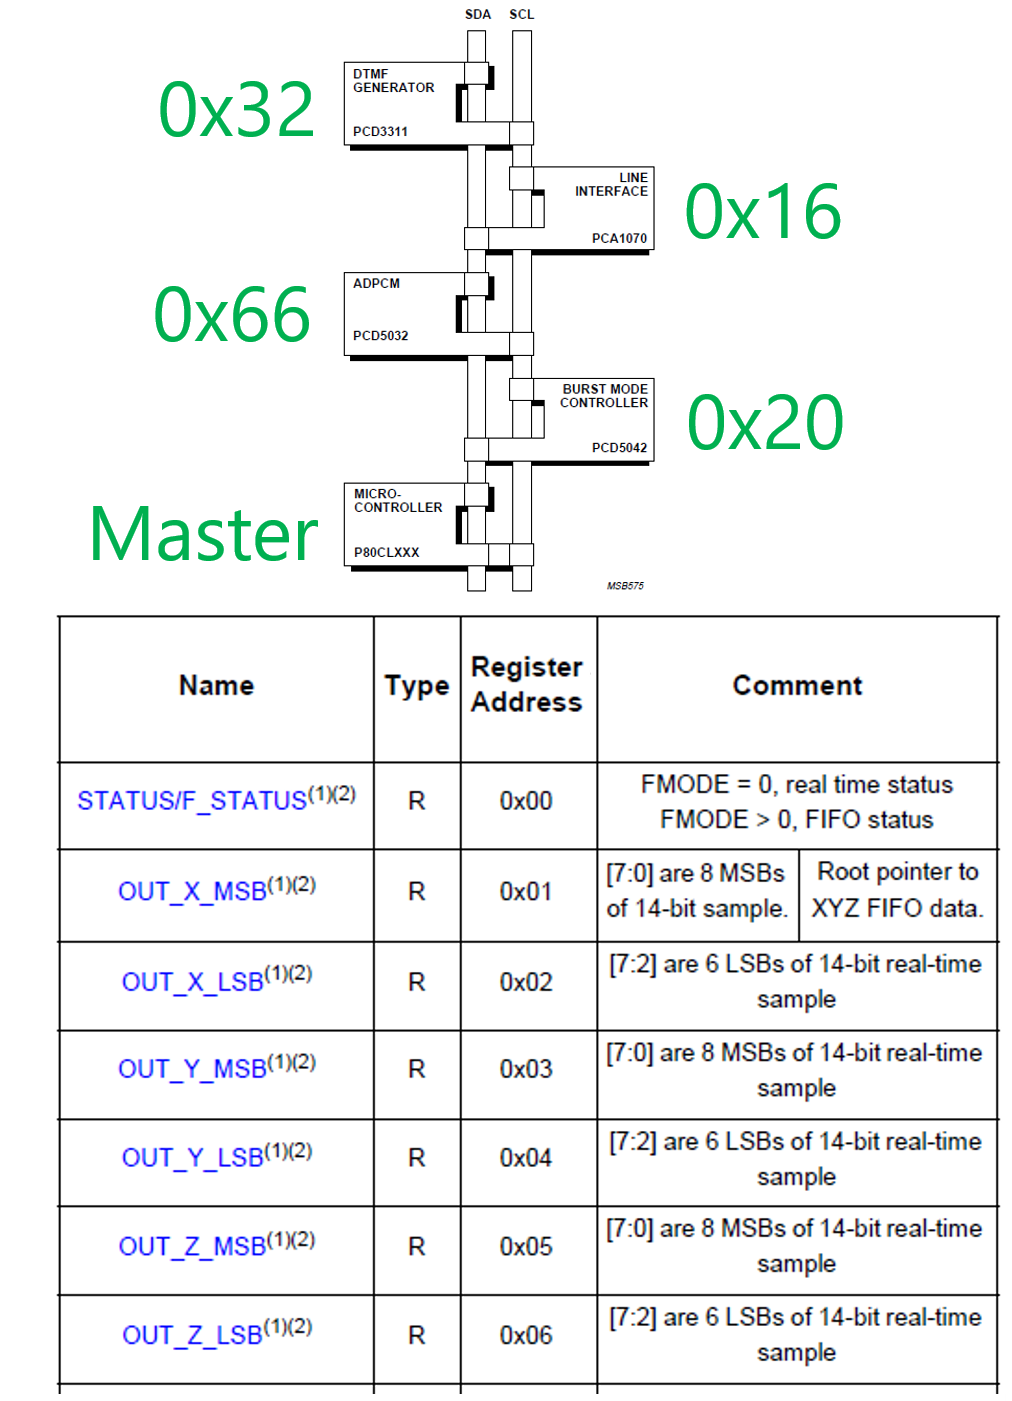
\includegraphics[scale=0.35]{24_I2CAddressing}
		\end{figure}
		
	\end{columns}	
	}
\end{frame}

%%%%%%%%%%%%%%%%% FRAME %%%%%%%%%%%%%%%%%%%%%%%%%%
\begin{frame}
	\frametitle{I2C - Direccionamiento a registros}
	{\small
		\begin{figure}
			\centering
			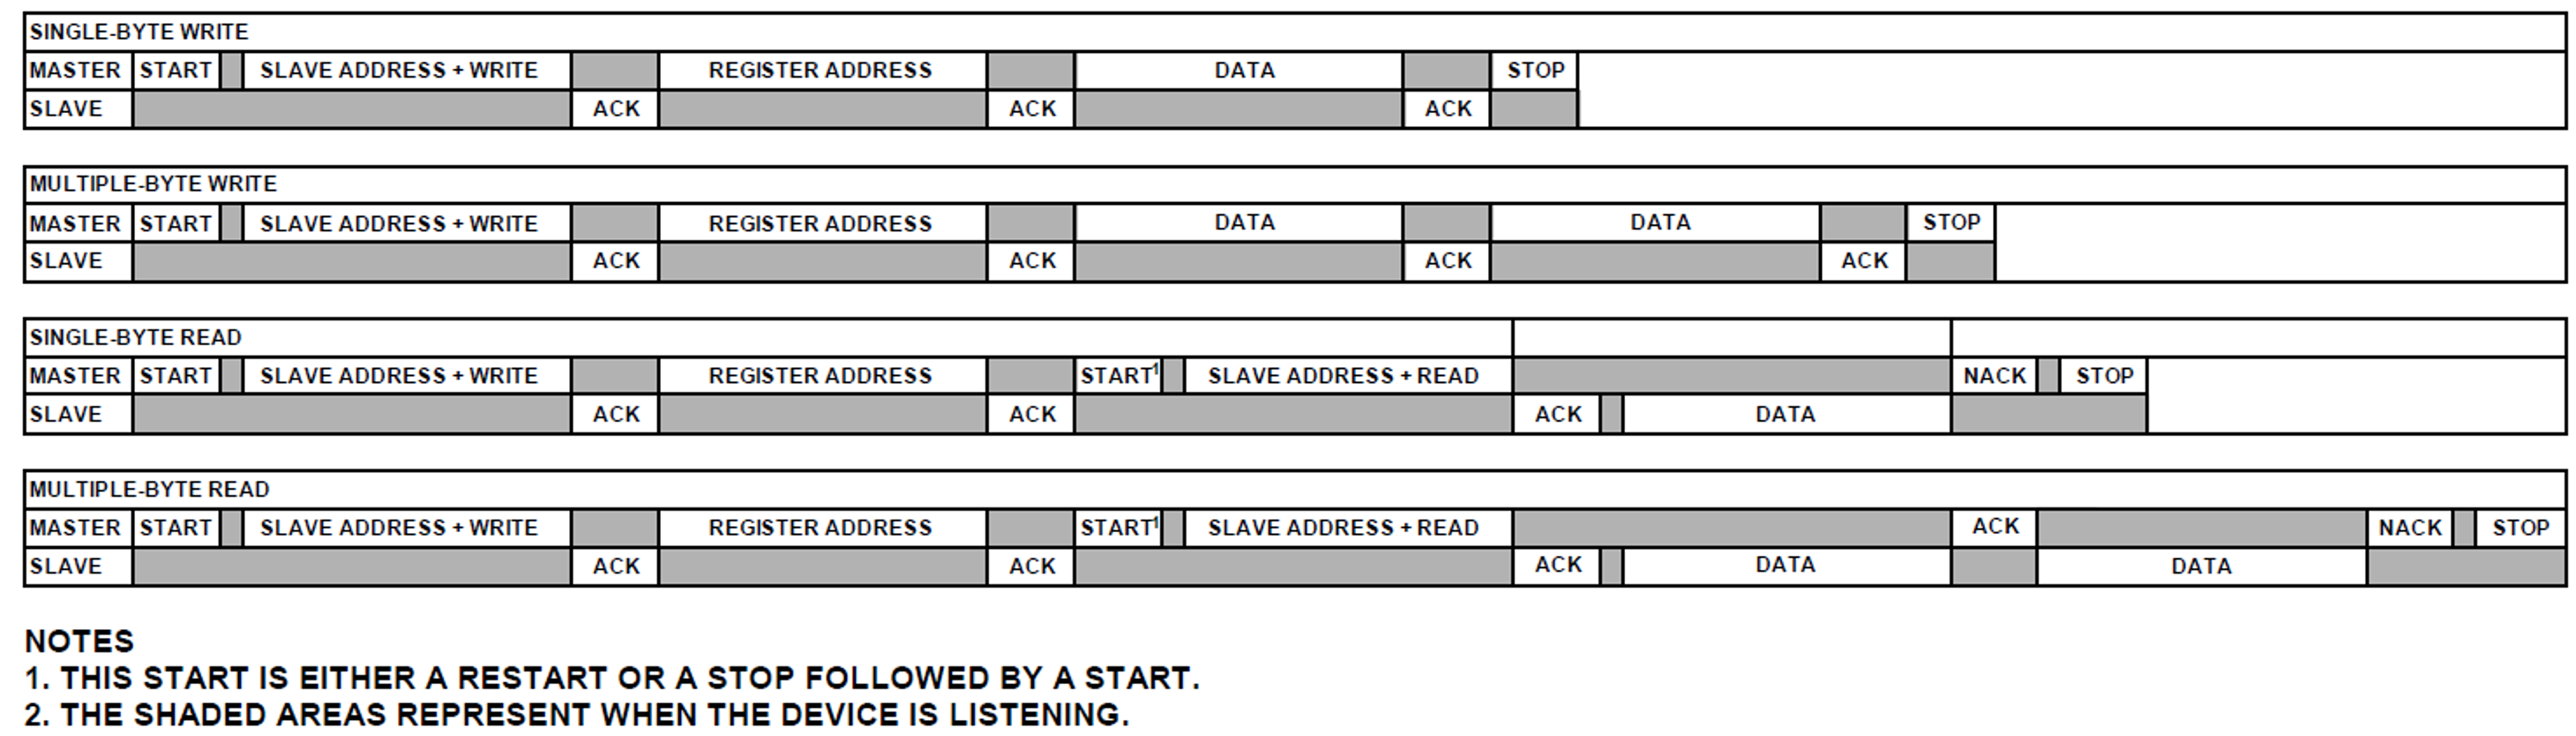
\includegraphics[scale=0.23]{25_I2CProtocol}
		\end{figure}
		
		\begin{itemize}
			\item La comunicación la dirige el maestro
			\begin{itemize}
				\item Se envía la condición de start, la dirección del esclavo, y el comando de lectura/escritura. 
				\item Se espera por el ACK del esclavo.
				\item Se envía el direccionamiento a registro. 
				\item Se espera el ACK del esclavo
			\end{itemize}
		\end{itemize}	
	}
\end{frame}
%%%%%%%%%%%%%%%%% FRAME %%%%%%%%%%%%%%%%%%%%%%%%%%
\begin{frame}
	\frametitle{I2C - Hardware}
	{\small
		\begin{figure}
			\centering
			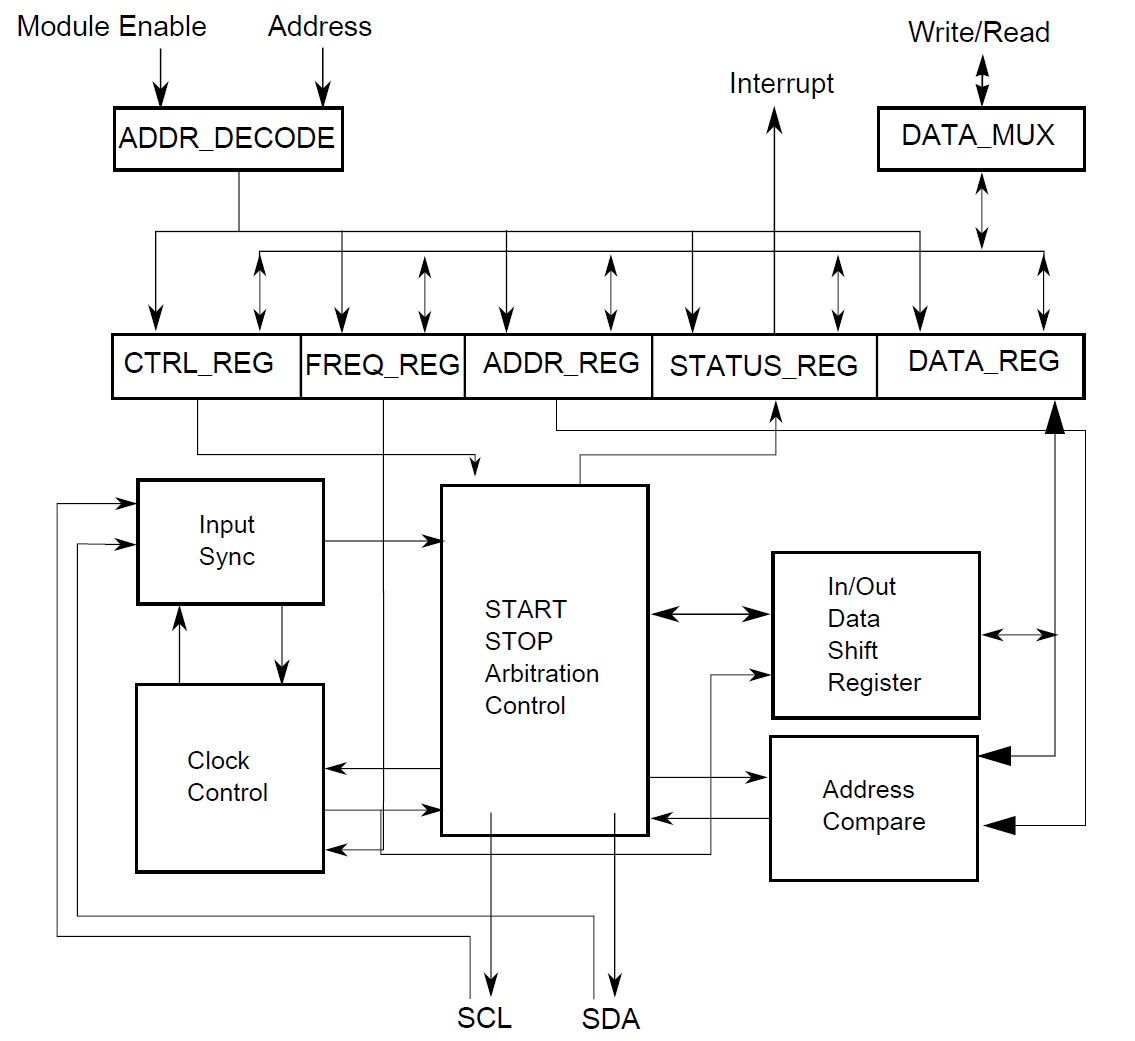
\includegraphics[scale=0.4]{26_I2CHardware}
		\end{figure}
	}
\end{frame}
%%%%%%%%%%%%%%%%% FRAME %%%%%%%%%%%%%%%%%%%%%%%%%%
\begin{frame}
	\frametitle{I2C - Configuración -  I2Cx\_F}
	{\small
		\begin{figure}
			\centering
			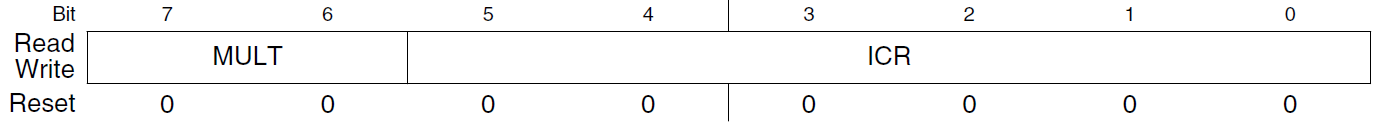
\includegraphics[scale=0.6]{27_I2CF}
		\end{figure}
		
		\begin{itemize}
			\item I2Cx\_F: registro de divisor de frecuencia
			\begin{itemize}
				\item MULT: especifica el multiplicador mul=$2^{\texttt{MULT}}$
				\item ICR: frecuencia del clock
				\item I2C baud rate: $f_{\texttt{bus}}/ (2^{\texttt{MULT}} * \texttt{ICR}) $
			\end{itemize}
		\end{itemize}	
	}
\end{frame}

%%%%%%%%%%%%%%%%% FRAME %%%%%%%%%%%%%%%%%%%%%%%%%%
\begin{frame}
	\frametitle{I2C - Configuración -  I2Cx\_C1}
	{\small
		\begin{figure}
			\centering
			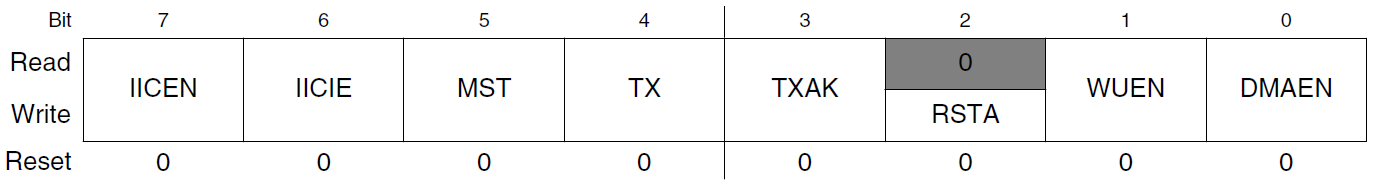
\includegraphics[scale=0.6]{28_I2CC1}
		\end{figure}
		
		\begin{multicols}{2}
			\begin{itemize}
				\item IICEN - habilita el I2C
				\item IICIE - habilita la interrupción del I2C
				\item MST - selecciona como modo maestro
				\begin{itemize}
					\item 0 a 1, genera la condición de start
					\item 1 a 0, genera la condición de stop
				\end{itemize}
				\item TX - selecciona 1 para transmitir desde el maestro y 0 para recibir
				\item TXAK - habilitar el ACK
				\item RSTA - repetir start
				\item WUEN - habilitar wakeup
				\item DMAEN - habilitar DMA
			\end{itemize}
		\end{multicols}
			
	}
\end{frame}
%%%%%%%%%%%%%%%%% FRAME %%%%%%%%%%%%%%%%%%%%%%%%%%
\begin{frame} 
	\frametitle{I2C - Configuración -  I2Cx\_S}
	{\small
		\begin{figure}
			\centering
			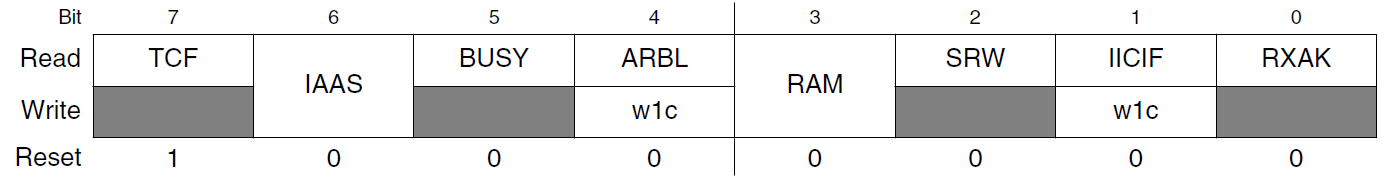
\includegraphics[scale=0.6]{29_I2CS}
		\end{figure}
		
		\begin{multicols}{2}
			\begin{itemize}
				\item TCF - bandera de transferencia completa, después de transmitir byte y ACK
				\item IAAS - direccionamiento como esclavo
				\item BUSY - bus ocupado
				\item ARBL - se pierde arbitración
				\item RAM - rango de direccionamiento alcanzado
				\item RXAK - señal ACK recibida
			\end{itemize}
		\end{multicols}
		
	}
\end{frame}
%%%%%%%%%%%%%%%%% FRAME %%%%%%%%%%%%%%%%%%%%%%%%%%
\begin{frame} 
	\frametitle{I2C - Configuración -  I2Cx\_D}
	{\small
		\begin{figure}
			\centering
			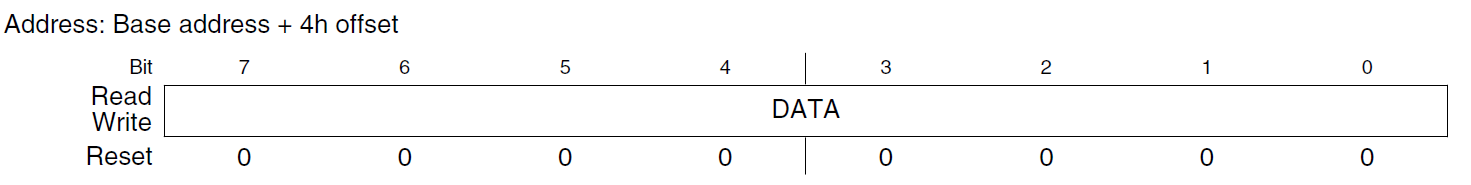
\includegraphics[scale=0.5]{30_I2CD}
		\end{figure}
		

			\begin{itemize}
				\item Registro de datos de 8 bits.
				\item Modo de transmisión maestro
				\begin{itemize}
					\item Escribir a este registro inicia la transferencia de datos.
				\end{itemize}
				\item Modo de recepción del maestro
				\begin{itemize}
					\item Leer este registro comienza la recepción del siguiente byte
				\end{itemize}
			\end{itemize}

		
	}
\end{frame}

%%%%%%%%%%%%%%%%% FRAME %%%%%%%%%%%%%%%%%%%%%%%%%%
\begin{frame}[fragile]
	\frametitle{I2C - Macros útiles}
	\begin{lstlisting}[style=CStyle]
#define I2C_M_START 	I2C0->C1 |= I2C_C1_MST_MASK
#define I2C_M_STOP  	I2C0->C1 &= ~I2C_C1_MST_MASK
#define I2C_M_RSTART	I2C0->C1 |= I2C_C1_RSTA_MASK

#define I2C_TRAN	I2C0->C1 |= I2C_C1_TX_MASK
#define I2C_REC		I2C0->C1 &= ~I2C_C1_TX_MASK

#define BUSY_ACK 	while(I2C0->S & 0x01)
#define TRANS_COMP	while(!(I2C0->S & 0x80))
#define I2C_WAIT	while((I2C0->S & I2C_S_IICIF_MASK)==0){} \                                 
							I2C0->S |= I2C_S_IICIF_MASK;

#define NACK	I2C0->C1 |= I2C_C1_TXAK_MASK
#define ACK    	I2C0->C1 &= ~I2C_C1_TXAK_MASK
		
	\end{lstlisting}
\end{frame}

%%%%%%%%%%%%%%%%% FRAME %%%%%%%%%%%%%%%%%%%%%%%%%%
\begin{frame}[fragile]
	\frametitle{I2C - Funciones}
	{\small
		\begin{multicols}{2}
			Mandar un byte
			\begin{lstlisting}[style=CStyle]
				I2C_TRAN;			/*set to transmit mode */
				I2C_M_START;		/*send start	*/
				I2C0->D = dev;  	/*send dev address */
				I2C_WAIT;	 		/*wait for ack */
				
				I2C0->D = address;	/*send write address */
				I2C_WAIT;
				
				I2C0->D = data;		/*send data	*/
				I2C_WAIT;
				I2C_M_STOP;
			\end{lstlisting}
			
			Leer un byte
			\begin{lstlisting}[style=CStyle]
				I2C_TRAN;	/*set to transmit mode */
				I2C_M_START;	/*send start	*/
				I2C0->D = dev;	/*send dev address	*/
				I2C_WAIT;	/*wait for completion */
				I2C0->D = address;	/*send read address */
				I2C_WAIT;	/*wait for completion */
				I2C_M_RSTART;	/*repeated start */
				I2C0->D = (dev|0x1); 	/*send dev address (read) */
				I2C_WAIT;	/*wait for completion */
				I2C_REC;	/*set to recieve mode */
				NACK;	/*set NACK after read	*/
				data = I2C0->D;	/*dummy read	*/
				I2C_WAIT;	/*wait for completion */
				I2C_M_STOP;	/*send stop	*/
				data = I2C0->D;	/*read data	*/
				
			\end{lstlisting}
		\end{multicols}
}
\end{frame}

%%%%%%%%%%%%%%%%% FRAME %%%%%%%%%%%%%%%%%%%%%%%%%%
\begin{frame}
	\frametitle{I2C - Ejemplo}
	{\small
		Se requiere tomar la temperatura y la humedad utilizando el sensor SHT3X cada segundo. 
		
		\textbf{Solución}:
		
		\begin{itemize}
			\item Configurar Clocks del sistema
			\item Configurar pines a utilizar
			\item Configurar los periféricos tanto del I2C como del PIT
			\item Configurar interrupción
			\item Hacer funciones para generar comandos al sensor.
		\end{itemize}
	}
\end{frame}
%%%%%%%%%%%%%%%%% FRAME %%%%%%%%%%%%%%%%%%%%%%%%%%
\begin{frame}
	\frametitle{I2C - Ejemplo - Solución}
	\begin{figure}
		\centering
		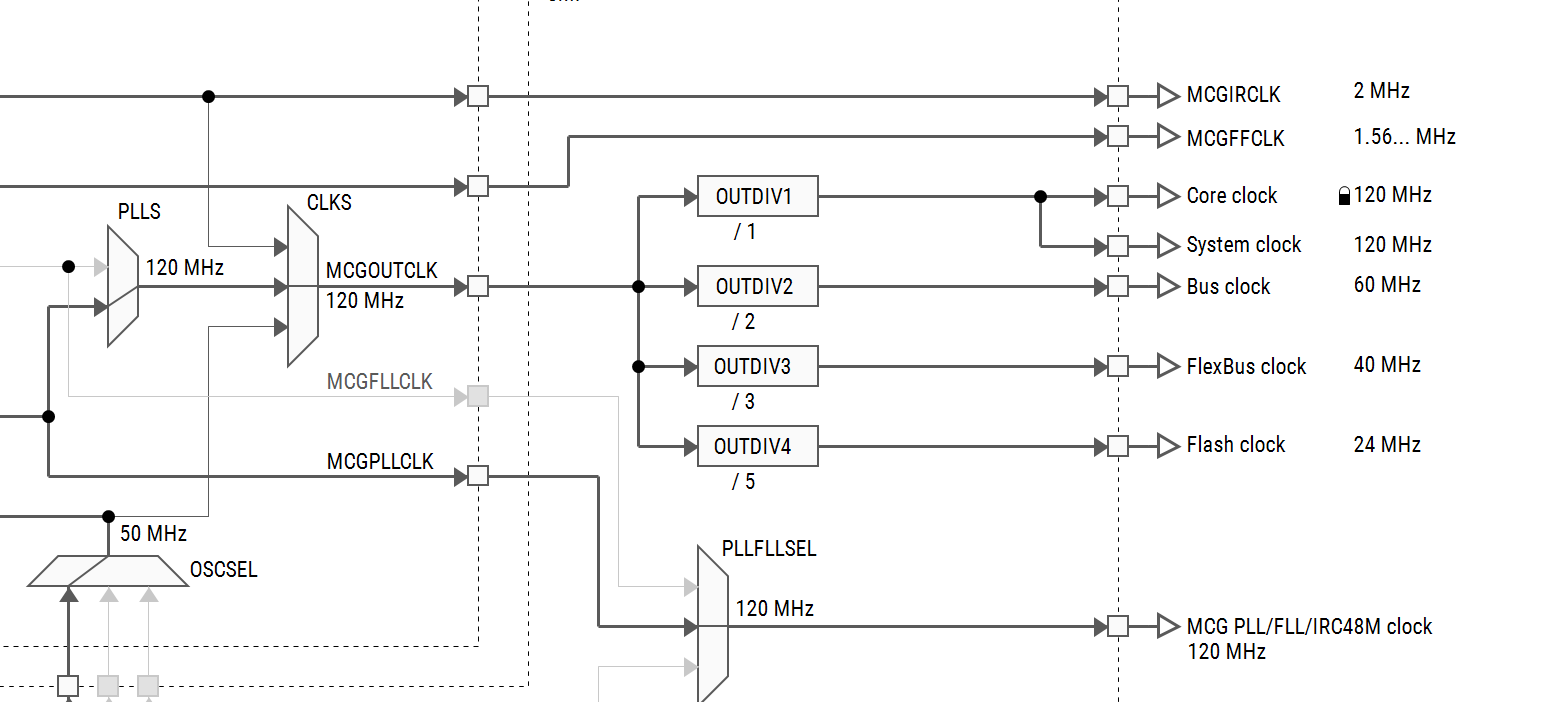
\includegraphics[scale=0.5]{19_ClockConfig}
	\end{figure}
\end{frame}
%%%%%%%%%%%%%%%%% FRAME %%%%%%%%%%%%%%%%%%%%%%%%%%
\begin{frame}
	\frametitle{I2C - Ejemplo - Solución}
	\begin{figure}
		\centering
		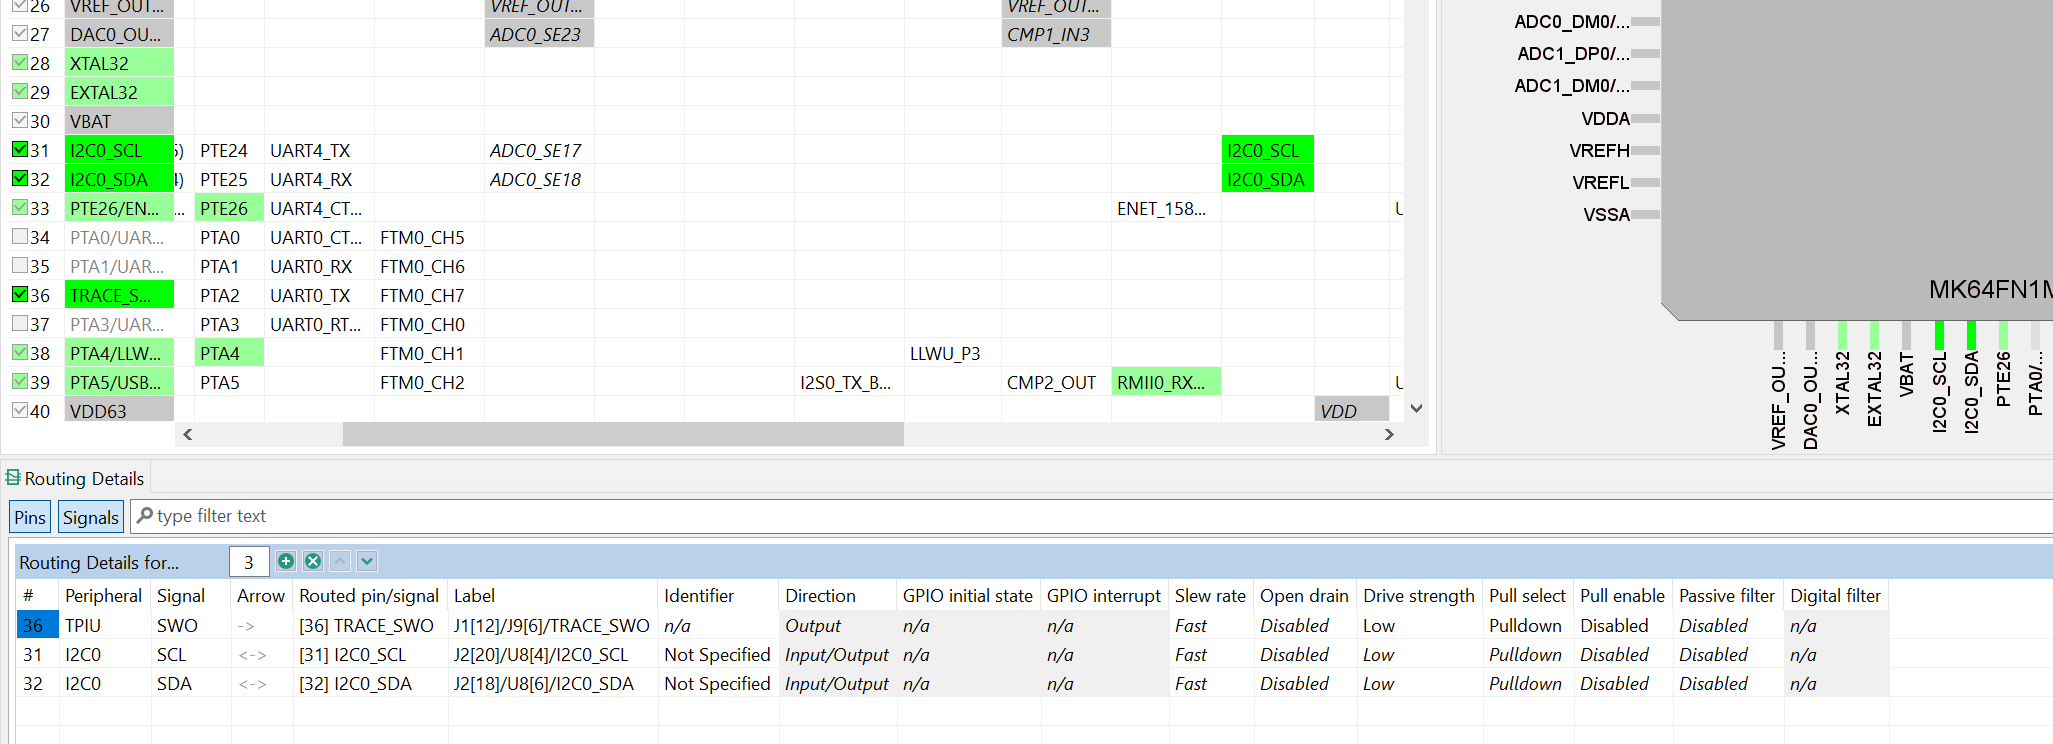
\includegraphics[scale=0.35]{31_I2CConfig}
	\end{figure}
\end{frame}

%%%%%%%%%%%%%%%%% FRAME %%%%%%%%%%%%%%%%%%%%%%%%%%
\begin{frame}
	\frametitle{I2C - Ejemplo - Solución}
	\begin{figure}
		\centering
		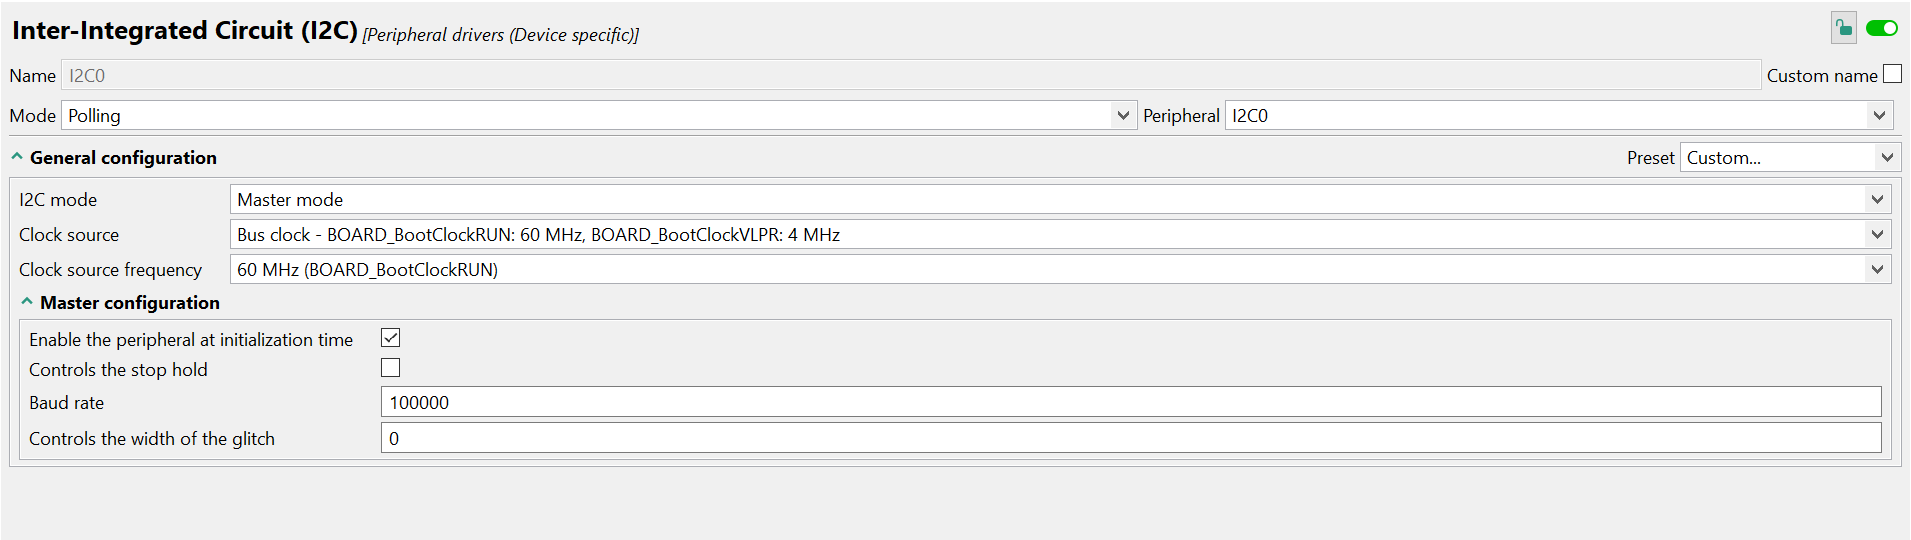
\includegraphics[scale=0.35]{32_I2CSetup}
	\end{figure}
\end{frame}

%%%%%%%%%%%%%%%%% FRAME %%%%%%%%%%%%%%%%%%%%%%%%%%
\begin{frame}
	\frametitle{I2C - Ejemplo - Solución}
	\begin{figure}
		\centering
		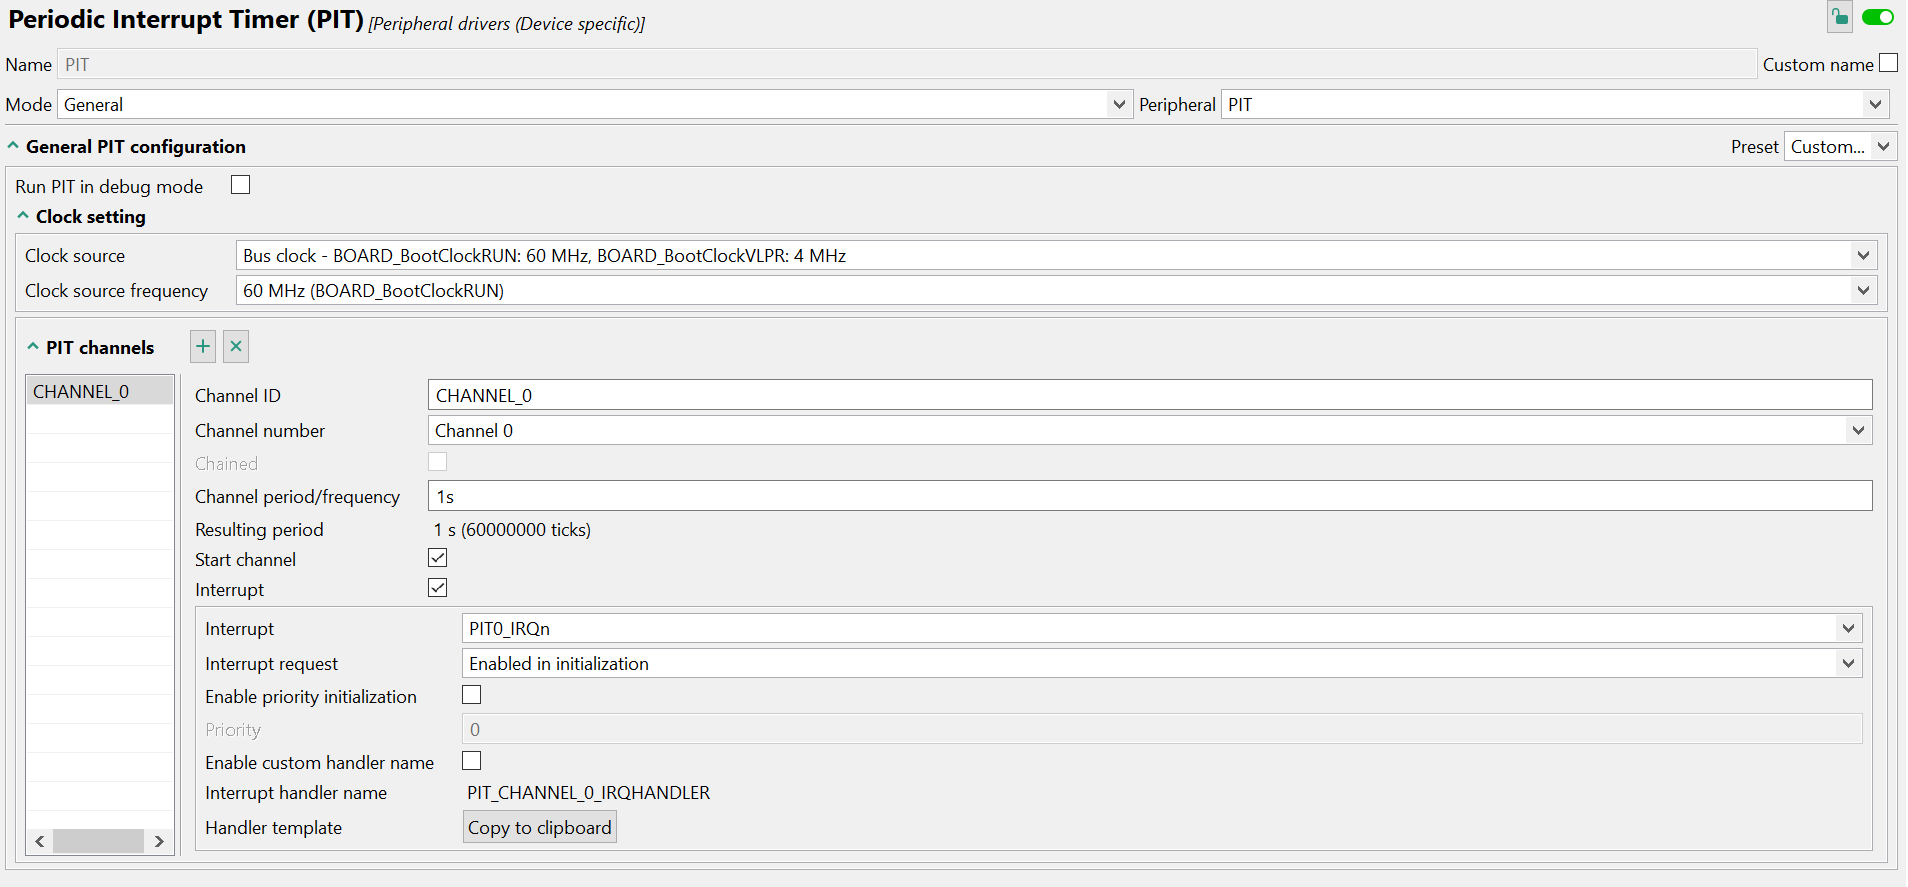
\includegraphics[scale=0.35]{33_PITConfig}
	\end{figure}
\end{frame}
%%%%%%%%%%%%%%%%% FRAME %%%%%%%%%%%%%%%%%%%%%%%%%%
\begin{frame}[fragile]
	\frametitle{I2C - Ejemplo - Solución}
	{\tiny
		Creación de algunas MACROS
		\begin{lstlisting}[style=CStyle]
#define SHT31_DEFAULT_ADDR          0x44U
#define SHT31_MEAS_HIGHREP          0x2400U
#define SHT31_MEAS_MEDREP           0x240BU
#define SHT31_MEAS_LOWREP           0x2416
#define SHT31_READSTATUS            0xF32D
#define SHT31_SOFTRESET             0x30A2U
#define I2C_Wait()					while((I2C_MasterGetStatusFlags(I2C0) & I2C_S_IICIF_MASK)==0) {} \
											I2C0->S |= I2C_S_IICIF_MASK;
		\end{lstlisting}
	
		Creación de función para envió de comando.
		\begin{lstlisting}[style=CStyle]
void writeCommand(uint16_t cmd, uint8_t address) {
	uint8_t buf[2];
	buf[0] = (cmd >> 8);
	buf[1] = (cmd & 0xFF);
	
	I2C_MasterStart(I2C0, address, kI2C_Write);							// Start transmission with Slave, write mode
	I2C_Wait(); 														// Wait for ACK
	I2C_MasterWriteBlocking(I2C0, buf, 2, kI2C_TransferDefaultFlag);	// Send command
}
		\end{lstlisting}
	
	Creación de función para soft reset.
	\begin{lstlisting}[style=CStyle]
void reset(void) {
	writeCommand(SHT31_SOFTRESET,SHT31_DEFAULT_ADDR);
	delaySimple(10000);
}
	\end{lstlisting}
	}
\end{frame}
%%%%%%%%%%%%%%%%% FRAME %%%%%%%%%%%%%%%%%%%%%%%%%%
\begin{frame}[fragile]
	\frametitle{I2C - Ejemplo - Solución}
	{\tiny
		Lectura de status
		\begin{lstlisting}[style=CStyle]
uint16_t readStatus(uint8_t address) {
	//Send command read status
	writeCommand(SHT31_READSTATUS,SHT31_DEFAULT_ADDR);
	
	// Read status
	uint8_t readbuffer[3];
	I2C_MasterStart(I2C0, address, kI2C_Read);	// Start transmission with Slave, read mode
	I2C_Wait();	// Wait for ACK
	I2C_MasterReadBlocking(I2C0, &readbuffer[0], 3, kI2C_TransferDefaultFlag); // read 3 data
	
	uint16_t stat = readbuffer[0];
	stat <<= 8;
	stat |= readbuffer[1];
	
	if (readbuffer[2] != crc8((uint8_t *) readbuffer, 2)) {
		PRINTF("CRC erroneo \r\n", stat);
		return false;
	}
	
	PRINTF("%d\r\n", stat);
	return stat;
}
		\end{lstlisting}		
	}
\end{frame}
%%%%%%%%%%%%%%%%% FRAME %%%%%%%%%%%%%%%%%%%%%%%%%%
\begin{frame}[fragile]
	\frametitle{I2C - Ejemplo - Solución}
	{\tiny
		Inicialización del sensor y CRC8
		\begin{lstlisting}[style=CStyle]
void Init_SHT3(void){
	reset();
	readStatus(SHT31_DEFAULT_ADDR);
}

uint8_t crc8(const uint8_t *data, int len) {
	uint8_t crc = 0xFF;
	size_t i, j;
	for (i = 0; i < len; i++) {
		crc ^= data[i];
		for (j = 0; j < 8; j++) {
			if ((crc & 0x80) != 0)
			crc = (uint8_t)((crc << 1) ^ 0x31);
			else
			crc <<= 1;
		}
	}
	return crc;
}

		\end{lstlisting}		
	}
\end{frame}
%%%%%%%%%%%%%%%%% FRAME %%%%%%%%%%%%%%%%%%%%%%%%%%
\begin{frame}[fragile]
	\frametitle{I2C - Ejemplo - Solución}
	{\tiny
		Lectura de temperatura y humedad
		\begin{multicols}{2}
			\begin{lstlisting}[style=CStyle]
_Bool readTempHum(void) {
	uint8_t readbuffer[6];
	
	writeCommand(SHT31_MEAS_HIGHREP,SHT31_DEFAULT_ADDR);
	
	delaySimple(500000);
	
	I2C_MasterStart(I2C0, SHT31_DEFAULT_ADDR, kI2C_Read);
	I2C_Wait();	// Wait for ACK
	I2C_MasterReadBlocking(I2C0, &readbuffer[0], 6, kI2C_TransferDefaultFlag);
	
	uint16_t ST, SRH;
	ST = readbuffer[0];
	ST <<= 8;
	ST |= readbuffer[1];
	
	if (readbuffer[2] != crc8((uint8_t *) readbuffer, 2)) {
		return false;
	}
	
	SRH = readbuffer[3];
	SRH <<= 8;
	SRH |= readbuffer[4];
	
	if (readbuffer[5] != crc8((uint8_t *) readbuffer+3, 2)) {
		return false;
	}
	
	double stemp = ST;
	stemp *= 175;
	stemp /= 0xffff;
	stemp = -45 + stemp;
	
	
	double shum = SRH;
	shum *= 100;
	shum /= 0xFFFF;
	
	PRINTF("La temperatura fue de: %f y la humedad de %f\n\r",stemp,shum);
	return true;
}
				
			\end{lstlisting}		
		\end{multicols}
		
	}
\end{frame}
%%%%%%%%%%%%%%%%% FRAME %%%%%%%%%%%%%%%%%%%%%%%%%%
\frame{
	\begin{center}
		\vspace{3cm}
		\LARGE \textcolor{blue}{SERIAL ASINCRÓNICO UART \\ (Universal Asynchronous Receiver-Transmitter)}
	\end{center}
}
%%%%%%%%%%%%%%%%% FRAME %%%%%%%%%%%%%%%%%%%%%%%%%%
\begin{frame}
	\frametitle{UART - Conceptos básicos transmisión}
	
	\begin{figure}
		\centering
		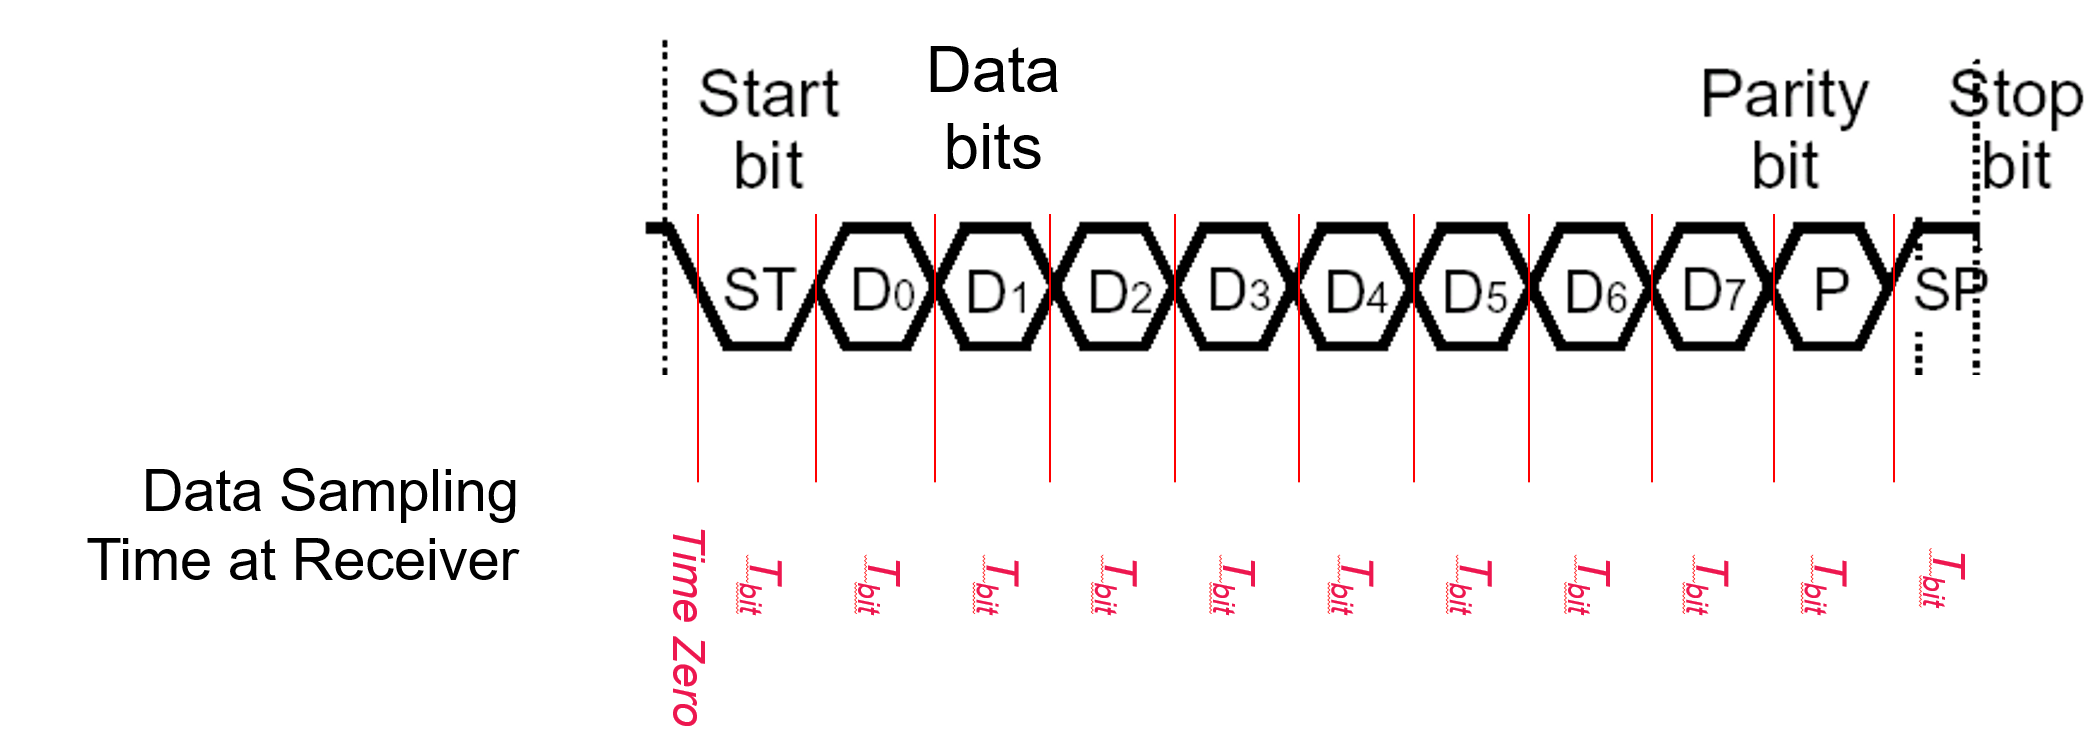
\includegraphics[scale=0.3]{34_UARTConcepts}
	\end{figure}
	
	\begin{itemize}
		\item Si no hay datos para enviar, la línea se mantiene en uno.
		\item Cuando se necesita enviar un datos, entonces:
		\begin{itemize}
			\item Se envia un cero, o start bit; para indicar el inicio de una transmisión.
			\item Enviar cada bit en la palabra (utiliza registros de desplazamiento).
			\item Envia un 1 para indicar el paro de la transmisión.
		\end{itemize}
	\end{itemize}
\end{frame}
%%%%%%%%%%%%%%%%% FRAME %%%%%%%%%%%%%%%%%%%%%%%%%%
\begin{frame}
	\frametitle{UART - Conceptos básicos recepción}
	
	\begin{figure}
		\centering
		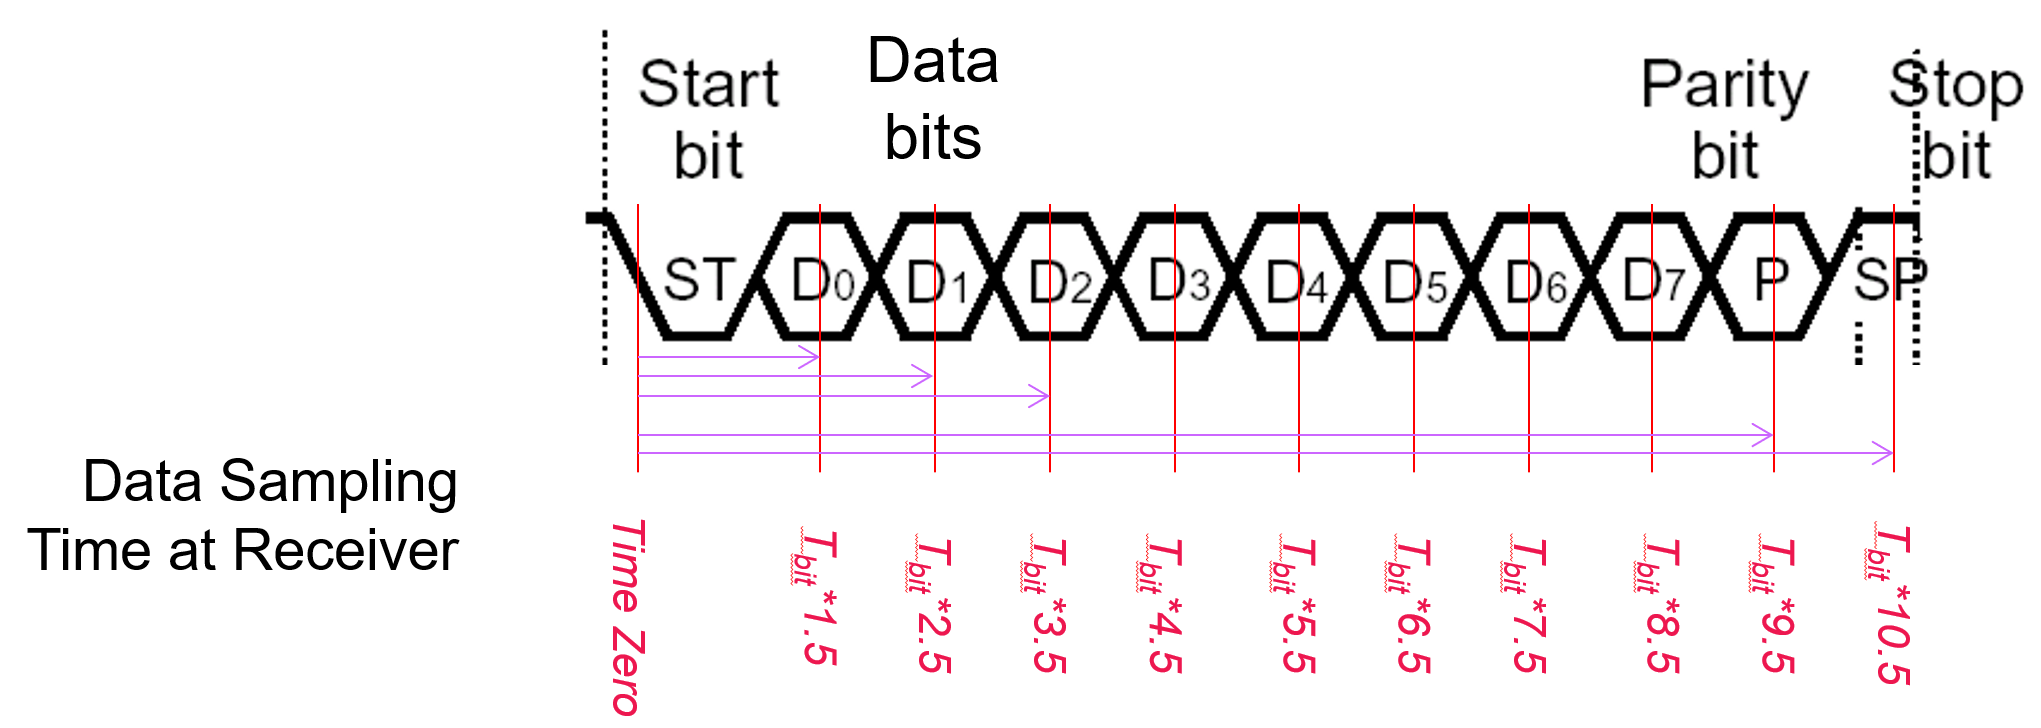
\includegraphics[scale=0.3]{35_UARTReceive}
	\end{figure}
	
	\begin{itemize}
		\item Se espera por un flanco de bajada.
		\begin{itemize}
			\item Se espera medio bit para tomar el dato
			\item Hacer lo siguiente de acuerdo a la cantidad de bits en la palabra
			\begin{itemize}
				\item Esperar un tiempo de un bit
				\item Leer el bit y desplazarlo al buffer de entrada
			\end{itemize}
			\item Esperar un bit
			\item Leer el bit: si es uno, entonces se acaba la transmisión. Si es cero, hay problemas. 
		\end{itemize}
	\end{itemize}
\end{frame}
%%%%%%%%%%%%%%%%% FRAME %%%%%%%%%%%%%%%%%%%%%%%%%%
\begin{frame}
	\frametitle{UART - Que se debe cumplir para que funcione?}
	\begin{itemize}
		\item El transmisor y el receptor deben coincidir en las mismas configuraciones:
		\begin{itemize}
			\item El orden de los bit de datos.
			\item Numero de bits de datos a transmitir
			\item Como es el bit de start y el bit de stop
			\item Cuanto dura un bit
			\item El transmisor y receptor deben tener clock muy parecidos ya que la única referencia es cuando se da el flanco en la bit de start
			\item En el K64 de 100 pines se tienen 5 UART
		\end{itemize}
	\end{itemize}
\end{frame}
%%%%%%%%%%%%%%%%% FRAME %%%%%%%%%%%%%%%%%%%%%%%%%%
\begin{frame}
	\frametitle{UART - Transmisor}
	
	\begin{figure}
		\centering
		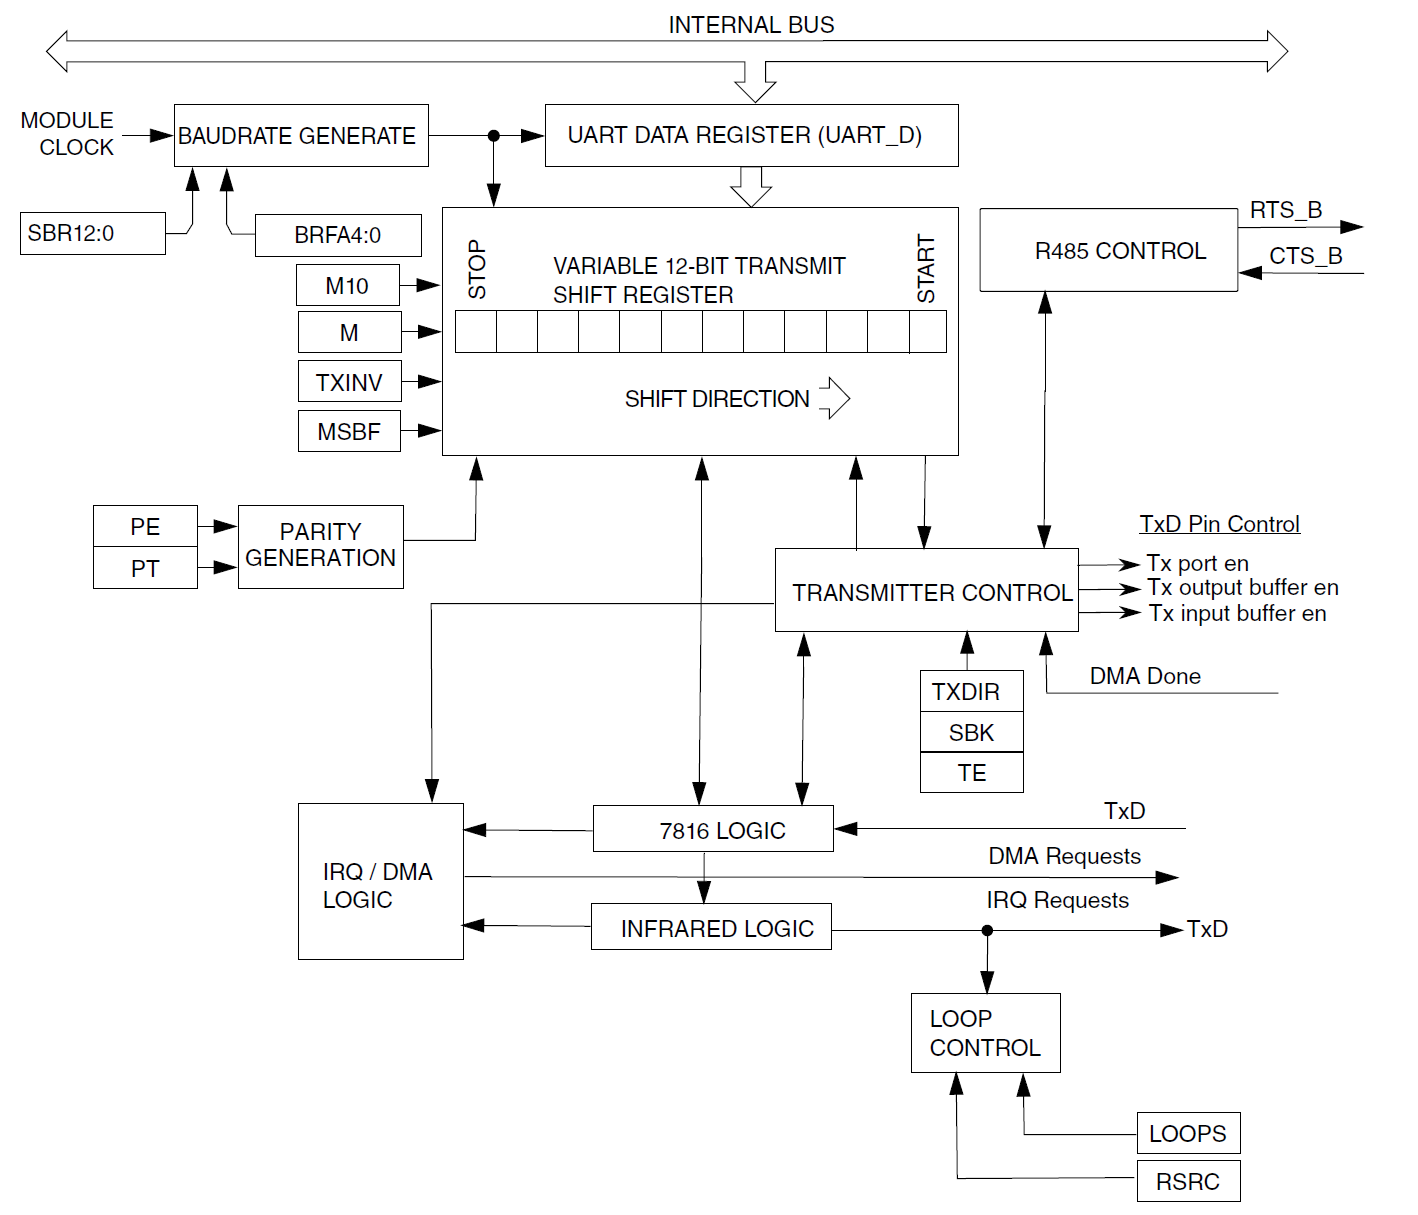
\includegraphics[scale=0.35]{36_UARTTransmitter}
	\end{figure}
\end{frame}
%%%%%%%%%%%%%%%%% FRAME %%%%%%%%%%%%%%%%%%%%%%%%%%
\begin{frame}
	\frametitle{UART - Receptor}
	
	\begin{figure}
		\centering
		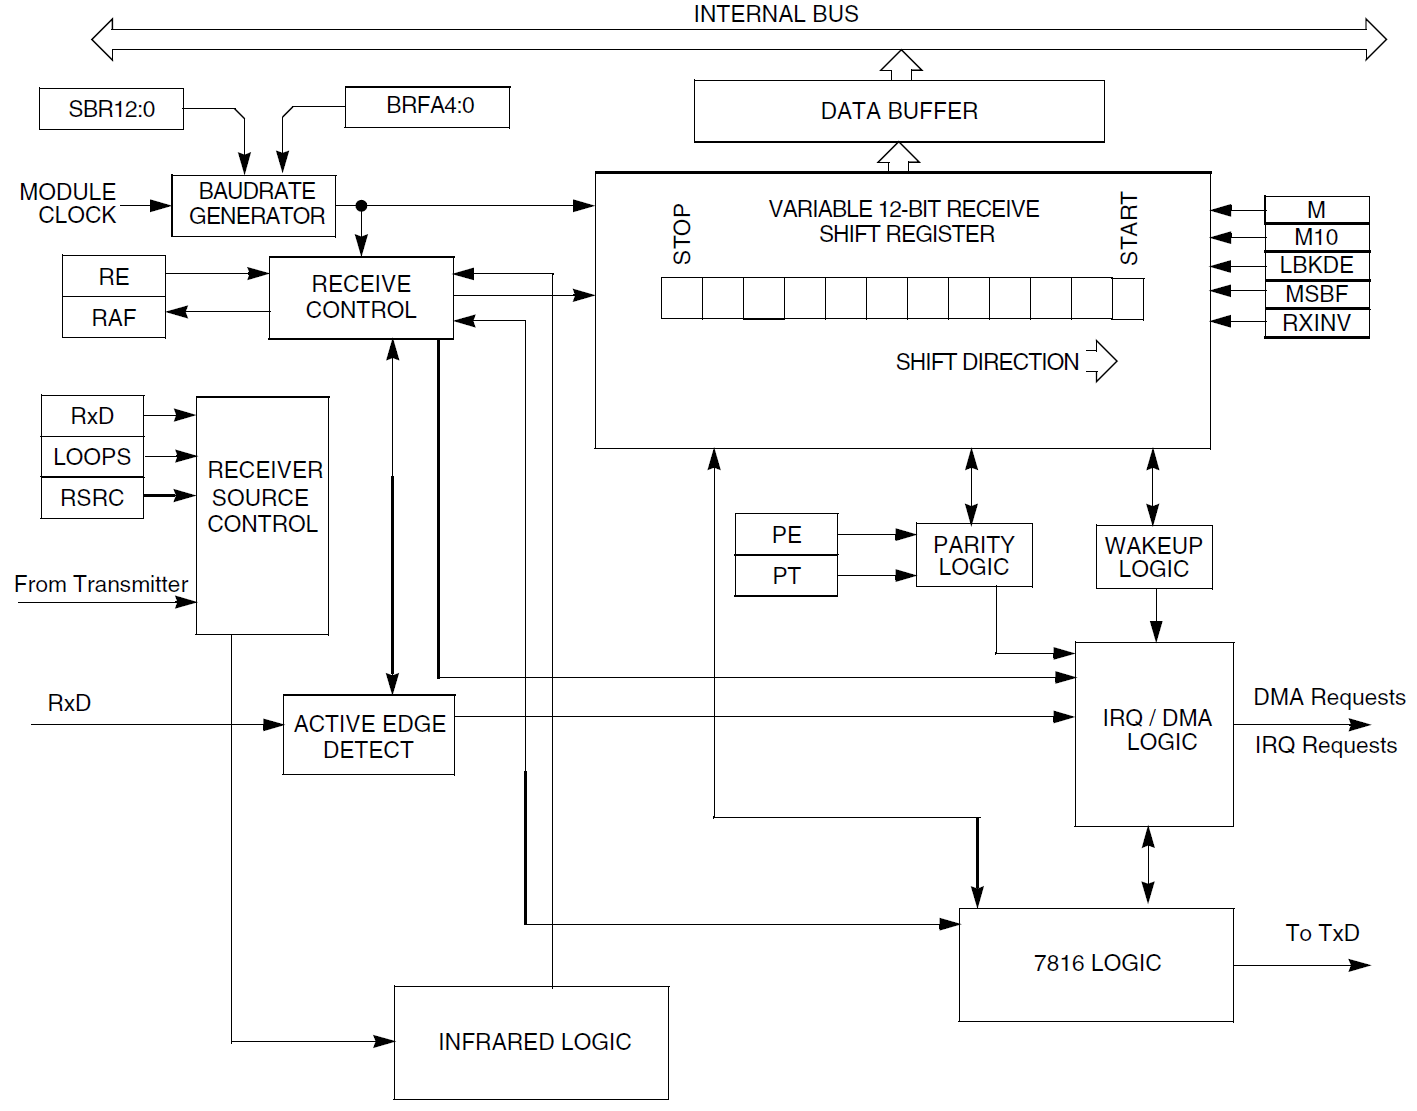
\includegraphics[scale=0.35]{37_UARTReceiver}
	\end{figure}
\end{frame}

%%%%%%%%%%%%%%%%% FRAME %%%%%%%%%%%%%%%%%%%%%%%%%%
\begin{frame}
	\frametitle{UART - Sobremuestreo}
	
	\begin{figure}
		\centering
		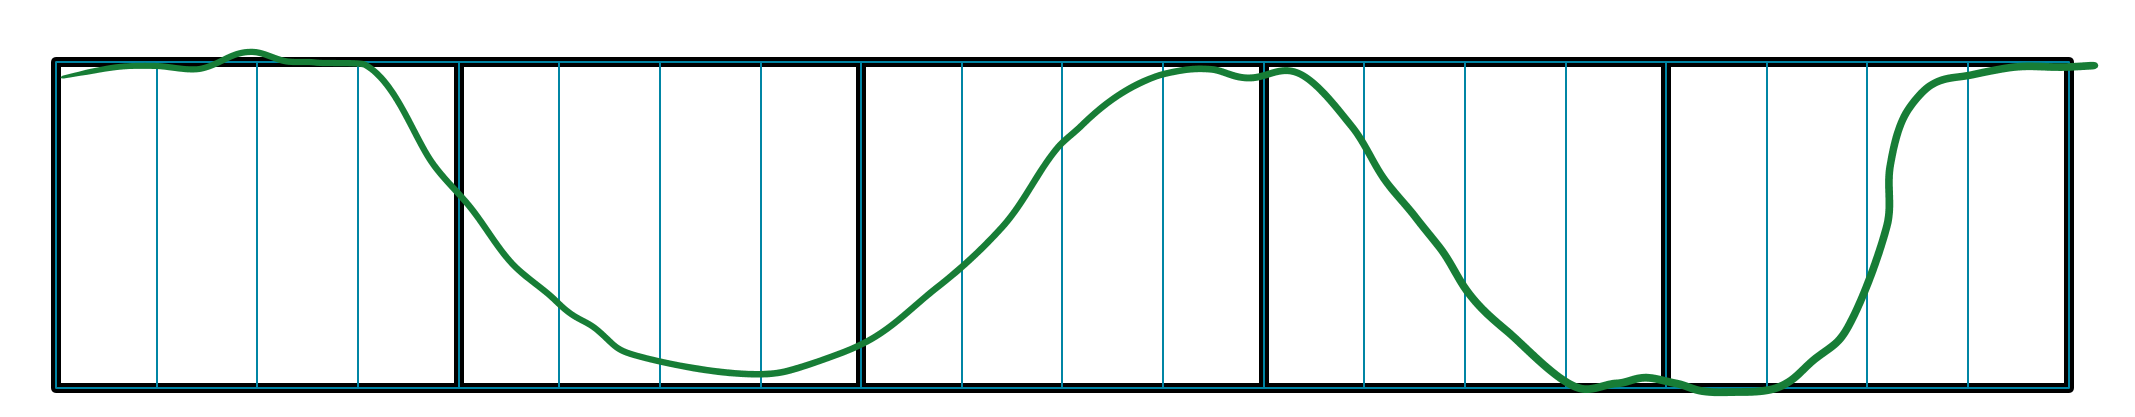
\includegraphics[scale=0.3]{38_UARTOverSampling}
	\end{figure}
	
	\begin{itemize}
		\item Cuando se recibe, el UART sobremuestrea la linea de datos
		\begin{itemize}
			\item Mas muestras permite botar y mejorar la inmunidad al ruido
			\item Mejor sincronización para la línea de datos
		\end{itemize}
		\item En el K64, el receptor muestrea la línea de acuerdo al RT clock, este RT clock es 16 veces el baud rate de la comunicación. 
	\end{itemize}
\end{frame}
%%%%%%%%%%%%%%%%% FRAME %%%%%%%%%%%%%%%%%%%%%%%%%%
\begin{frame}
	\frametitle{UART - Generador de clock}
	
	\begin{figure}
		\centering
		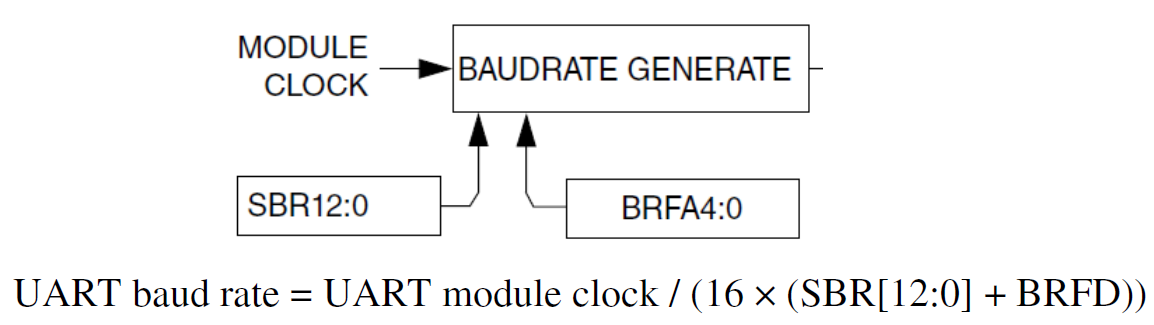
\includegraphics[scale=0.6]{39_UARTBaudRateGenerator}
	\end{figure}
	
	\begin{itemize}
		\item UART0 y UART 1 utilizan el clock del sistema (\SI{120}{\mega\hertz}), y UART2-4 el clock del bus (\SI{60}{\mega\hertz})
		\item Se requiere dividir la frecuencia del Bus para lograr el baud rate deseado 
		\item Ejemplo: se usa el UART2 con frecuencia de bus de 60MHz. Para lograr 9600 baud rate entonces
		\[
			SBR = 60E6/(9600*16) = 390
		\]
	\end{itemize}
\end{frame}
%%%%%%%%%%%%%%%%% FRAME %%%%%%%%%%%%%%%%%%%%%%%%%%
\begin{frame}
	\frametitle{UART - Registro UARTx\_C1}
	{\small
	\begin{figure}
		\centering
		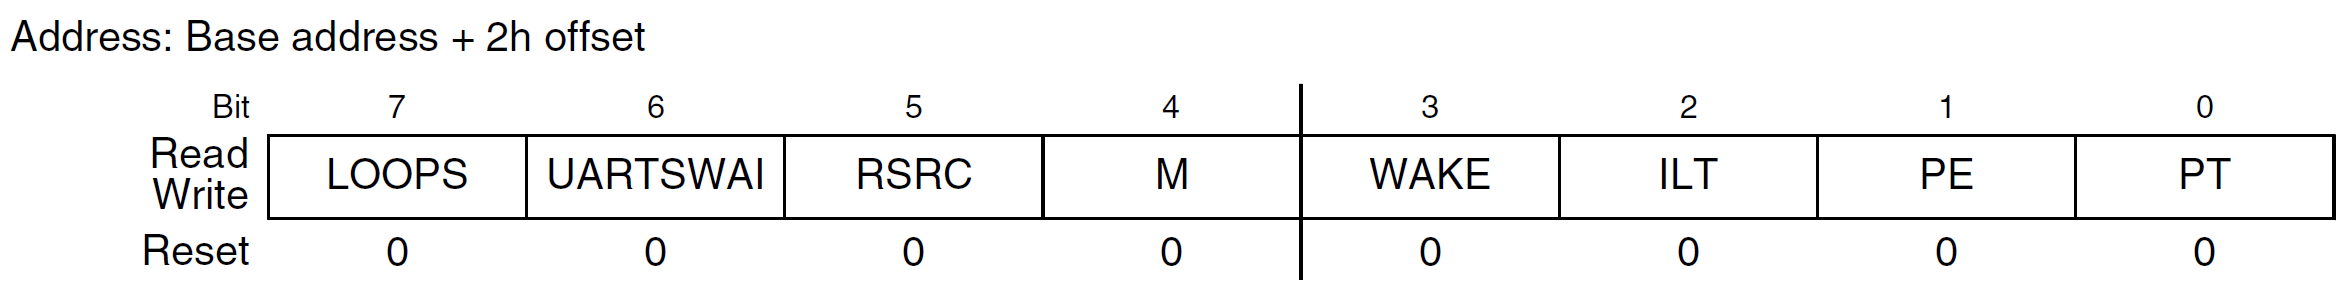
\includegraphics[scale=0.3]{40_UARTC1}
	\end{figure}
	
	\begin{itemize}
		\item LOOPS: habilita un loop interno entre Tx y Rx. 0 Operación normal 
		\item UARTSAWI: UART para en modo espera
		\item RSRC: seleccionar la fuente en loop
		\item M: Seleccionar datos de 9bits
		\item WAKE: método de despertar
		\item ILT: tipo de idle
		\item PE: paridad habilitada con 1
		\item PT: paridad impar con 1 y par con 0
	\end{itemize}
	}
\end{frame}
%%%%%%%%%%%%%%%%% FRAME %%%%%%%%%%%%%%%%%%%%%%%%%%
\begin{frame}
	\frametitle{UART - Registro UARTx\_C2}
	{\small
		\begin{figure}
			\centering
			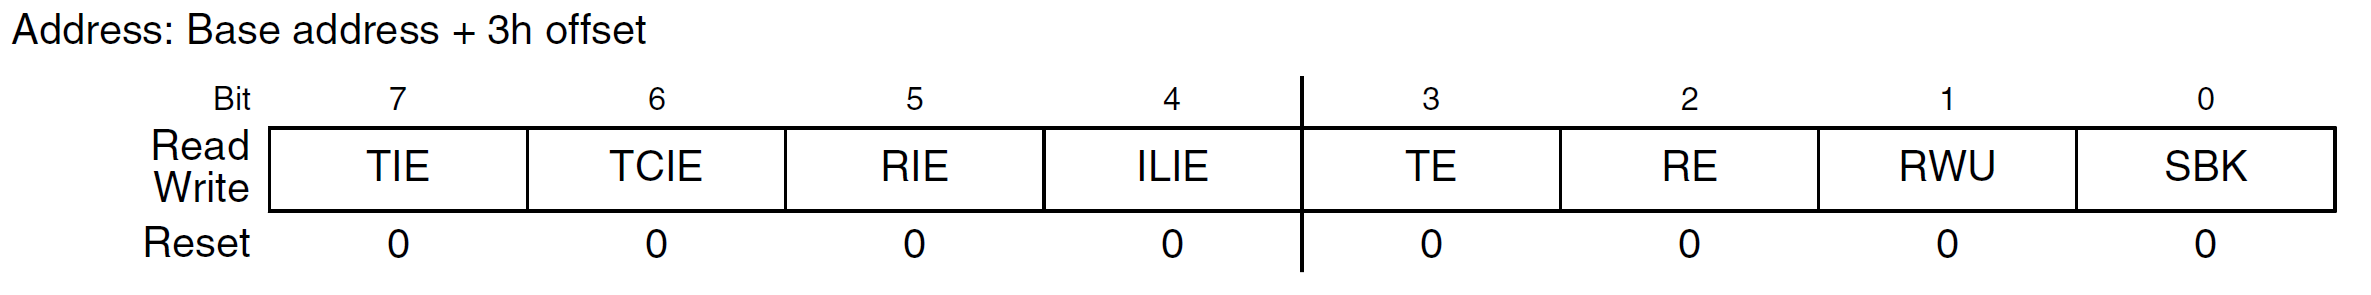
\includegraphics[scale=0.3]{41_UARTC2}
		\end{figure}
		
		\begin{itemize}
			\item Habilitar las interrupciones
			\begin{itemize}
				\item TIE: Interrupción cuando Tx esta vació.
				\item TCIE: interrupción cuando Tx está completo.
				\item RIE: interrupción cuando Rx tiene dato
			\end{itemize}
			\item Habilitar el módulo
			\begin{itemize}
				\item TE: Habilitar Tx
				\item RE: Habilitar Rx
			\end{itemize}
			\item Otros
			\begin{itemize}
				\item RWU: poner el receptor en modo espera, se despierta cuando ocurra el evento de despertar
				\item SBK: mandar un caracter de break (todos ceros)
			\end{itemize}
		\end{itemize}
	}
\end{frame}
%%%%%%%%%%%%%%%%% FRAME %%%%%%%%%%%%%%%%%%%%%%%%%%
\begin{frame}
	\frametitle{UART - Registro UARTx\_S1}
	{\small
		\begin{figure}
			\centering
			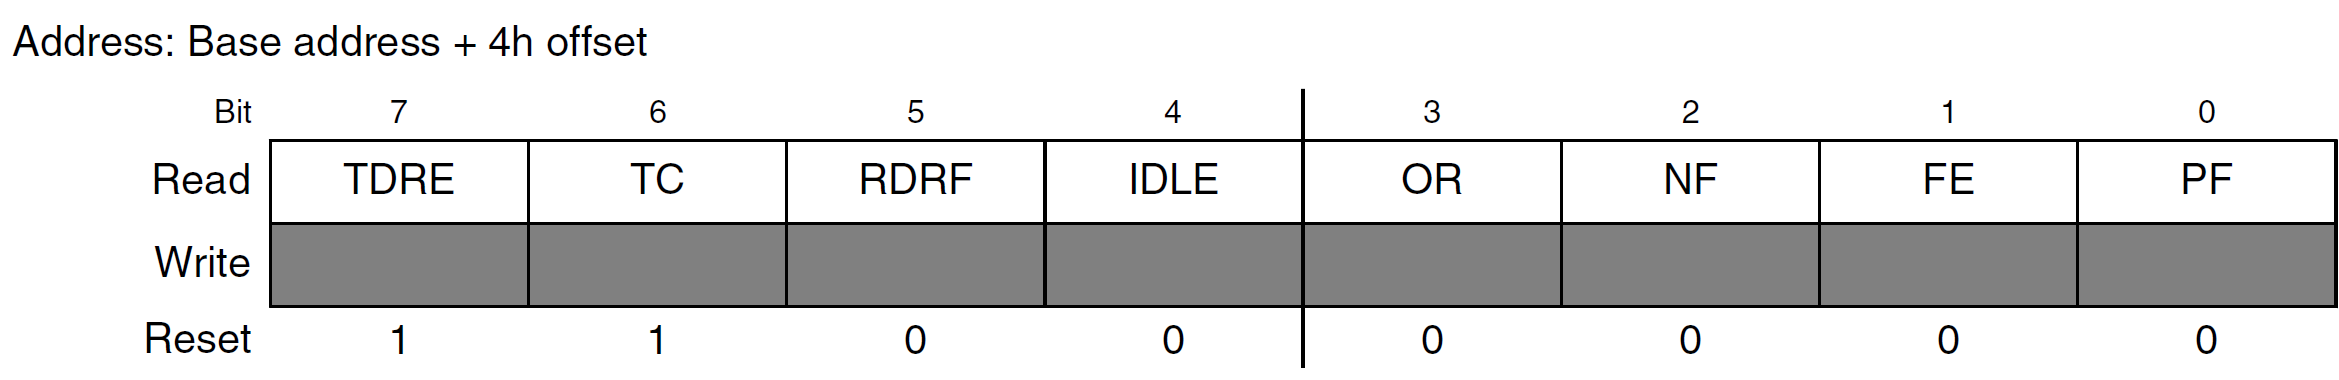
\includegraphics[scale=0.3]{42_UARTS1}
		\end{figure}
		
		\begin{itemize}
			\item TDRE: el registro de Tx está vació, puede escribir mas datos
			\item TC: Tx completada
			\item RDRF: Receptor lleno en el registro, puede recibir mas datos
			\item IDLE: UART se pone en idle durante un caracter
			\item OR: Se ha borrado el dato de recepción por uno nuevo
			\item NF: Bandera de ruido
			\item FE: Recibido un cero para parada y esperaba un uno
			\item PF: Error de paridad
		\end{itemize}
	}
\end{frame}
%%%%%%%%%%%%%%%%% FRAME %%%%%%%%%%%%%%%%%%%%%%%%%%
\begin{frame}
	\frametitle{UART - Registro UARTx\_S2}
	{\small
		\begin{figure}
			\centering
			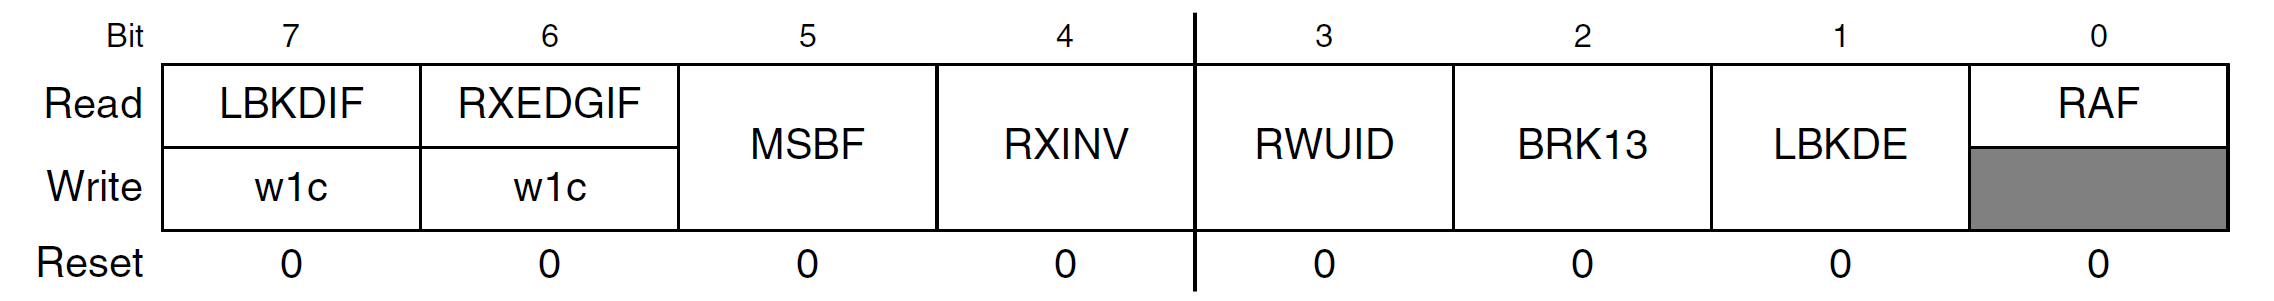
\includegraphics[scale=0.3]{43_UARTS2}
		\end{figure}
		
		\begin{itemize}
			\item LBKDIF: detecta la bandera de interrupción
			\item RXEDGIF: detecta flanco activo en el pin de recepción.
			\item MSBF: mandar el bit más significativo primero.
			\item RXINV: invertir la polaridad de las señales de recepción. 
			\item RWUID: activa bit de recepción para despertar el MCU.
			\item BRK13: envía carácter de break de acuerdo a la longitud.
			\item LBKDE: habilitar la linea break
			\item RAF: no hay linea idle
		\end{itemize}
	}
\end{frame}
%%%%%%%%%%%%%%%%% FRAME %%%%%%%%%%%%%%%%%%%%%%%%%%
\begin{frame}[fragile]
	\frametitle{UART - Polling Serial Comm}
	{\tiny
		\begin{lstlisting}[style=CStyle]
void Init_UART2(uint32_t baud_rate) {
	uint32_t divisor;
	// enable clock to UART and Port A
	SIM->SCGC4 |= SIM_SCGC4_UART2_MASK;
	SIM->SCGC5 |= SIM_SCGC5_PORTE_MASK;
	
	// connect UART to pins for PTE22, PTE23
	PORTE->PCR[22] = PORT_PCR_MUX(4);
	PORTE->PCR[23] = PORT_PCR_MUX(4);
	// ensure tx and rx are disabled before configuration
	UART2->C2 &=  ~(UARTLP_C2_TE_MASK | UARTLP_C2_RE_MASK);
	
	// Set baud rate
	divisor = BUS_CLOCK/(baud_rate*16);
	UART2->BDH = UART_BDH_SBR(divisor>>8);
	UART2->BDL = UART_BDL_SBR(divisor);
	
	// No parity, 8 bits, two stop bits, other settings;
	UART2->C1 = UART2->S2 = UART2->C3 = 0;
	
	// Enable transmitter and receiver
	UART2->C2 = UART_C2_TE_MASK | UART_C2_RE_MASK;	
}
		\end{lstlisting}		
	}
\end{frame}
%%%%%%%%%%%%%%%%% FRAME %%%%%%%%%%%%%%%%%%%%%%%%%%
\begin{frame}[fragile]
	\frametitle{UART - Transmisión serial}
	{\tiny
		\begin{lstlisting}[style=CStyle]
void UART2_Transmit_Poll(uint8_t data) {
	// wait until transmit data register is empty
	while (!(UART2->S1 & UART_S1_TDRE_MASK));
	UART2->D = data;
}	
void main(void) {
	char c;	
	// Initialization goes here
	while (1) {
		for (c='a'; c<='z'; c++) {
			UART2_Transmit_Poll(c);
		}
	}
}
		\end{lstlisting}		
	}
\end{frame}
%%%%%%%%%%%%%%%%% FRAME %%%%%%%%%%%%%%%%%%%%%%%%%%
\begin{frame}[fragile]
	\frametitle{UART - Recepción serial}
	{\tiny
		\begin{lstlisting}[style=CStyle]
uint8_t UART2_Receive_Poll(void) {
	// wait until receive data register is full
	while (!(UART2->S1 & UART_S1_RDRF_MASK));
	return UART2->D;
}	
void main(void) {
	char c;	
	// Initialization goes here
	while (1) {
		c = UART2_Receive_Poll();
		UART2_Transmit_Poll(c);
	}
}
		\end{lstlisting}		
	}
\end{frame}
%%%%%%%%%%%%%%%%% FRAME %%%%%%%%%%%%%%%%%%%%%%%%%%
\begin{frame}[fragile]
	\frametitle{UART - Inicialización e Interrupciones}
	{\small
		Usar interrupciones e inicializar periféricos para el MCU. El ISR debe identificar porque se genera la interrupción. 
		
		\begin{multicols}{2}
		\begin{lstlisting}[style=CStyle]
void Init_UART2(uint32_t baud_rate) {
	NVIC_SetPriority(UART2_IRQn, 2); 
	NVIC_ClearPendingIRQ(UART2_IRQn); 
	NVIC_EnableIRQ(UART2_IRQn);
	
	UART2->C2 |= UART_C2_TIE_MASK | 
	UART_C2_RIE_MASK;
	UART2->C2 |= UART_C2_RIE_MASK;
	Q_Init(&TxQ);
	Q_Init(&RxQ);
}
void UART2_IRQHandler(void) {
	NVIC_ClearPendingIRQ(UART2_IRQn);
	if (UART2->S1 & UART_S1_TDRE_MASK) {
		// can send another character
		if (!Q_Empty(&TxQ)) {
			UART2->D = Q_Dequeue(&TxQ);
		} else {
			// queue is empty so disable tx
			UART2->C2 &= ~UART_C2_TIE_MASK;
		}
	}
	if (UART2->S1 & UART_S1_RDRF_MASK) {
		// received a character
		if (!Q_Full(&RxQ)) {
			Q_Enqueue(&RxQ, UART2->D);
		} else {
			// error - queue full.
			while (1);
		}
	}	
}
		\end{lstlisting}	
		\end{multicols}
				
	}
\end{frame}
%%%%%%%%%%%%%%%%% FRAME %%%%%%%%%%%%%%%%%%%%%%%%%%
\frame{
\begin{center}
	\LARGE \textcolor{blue}{COMUNICACIONES SERIALES}
\end{center}

\begin{center}
	\LARGE \textcolor{blue}{GRACIAS}
\end{center}
}

%%%%%%%%%%%%%%%%%%%%%%%%%%%%%%%%%%%%%%%%%%%%%%%%%%%%%%%%%%%%%%%%%%%%%%%%%%%%%%%%%%%%%%%%%%%%%%%%%%%%%%%%%%%%%



\end{document}

